\documentclass[twoside]{book}

% Packages required by doxygen
\usepackage{fixltx2e}
\usepackage{calc}
\usepackage{doxygen}
\usepackage[export]{adjustbox} % also loads graphicx
\usepackage{graphicx}
\usepackage[utf8]{inputenc}
\usepackage{makeidx}
\usepackage{multicol}
\usepackage{multirow}
\PassOptionsToPackage{warn}{textcomp}
\usepackage{textcomp}
\usepackage[nointegrals]{wasysym}
\usepackage[table]{xcolor}

% NLS support packages
\usepackage[french]{babel}

% Font selection
\usepackage[T1]{fontenc}
\usepackage[scaled=.90]{helvet}
\usepackage{courier}
\usepackage{amssymb}
\usepackage{sectsty}
\renewcommand{\familydefault}{\sfdefault}
\allsectionsfont{%
  \fontseries{bc}\selectfont%
  \color{darkgray}%
}
\renewcommand{\DoxyLabelFont}{%
  \fontseries{bc}\selectfont%
  \color{darkgray}%
}
\newcommand{\+}{\discretionary{\mbox{\scriptsize$\hookleftarrow$}}{}{}}

% Page & text layout
\usepackage{geometry}
\geometry{%
  a4paper,%
  top=2.5cm,%
  bottom=2.5cm,%
  left=2.5cm,%
  right=2.5cm%
}
\tolerance=750
\hfuzz=15pt
\hbadness=750
\setlength{\emergencystretch}{15pt}
\setlength{\parindent}{0cm}
\setlength{\parskip}{3ex plus 2ex minus 2ex}
\makeatletter
\renewcommand{\paragraph}{%
  \@startsection{paragraph}{4}{0ex}{-1.0ex}{1.0ex}{%
    \normalfont\normalsize\bfseries\SS@parafont%
  }%
}
\renewcommand{\subparagraph}{%
  \@startsection{subparagraph}{5}{0ex}{-1.0ex}{1.0ex}{%
    \normalfont\normalsize\bfseries\SS@subparafont%
  }%
}
\makeatother

% Headers & footers
\usepackage{fancyhdr}
\pagestyle{fancyplain}
\fancyhead[LE]{\fancyplain{}{\bfseries\thepage}}
\fancyhead[CE]{\fancyplain{}{}}
\fancyhead[RE]{\fancyplain{}{\bfseries\leftmark}}
\fancyhead[LO]{\fancyplain{}{\bfseries\rightmark}}
\fancyhead[CO]{\fancyplain{}{}}
\fancyhead[RO]{\fancyplain{}{\bfseries\thepage}}
\fancyfoot[LE]{\fancyplain{}{}}
\fancyfoot[CE]{\fancyplain{}{}}
\fancyfoot[RE]{\fancyplain{}{\bfseries\scriptsize Généré par Doxygen }}
\fancyfoot[LO]{\fancyplain{}{\bfseries\scriptsize Généré par Doxygen }}
\fancyfoot[CO]{\fancyplain{}{}}
\fancyfoot[RO]{\fancyplain{}{}}
\renewcommand{\footrulewidth}{0.4pt}
\renewcommand{\chaptermark}[1]{%
  \markboth{#1}{}%
}
\renewcommand{\sectionmark}[1]{%
  \markright{\thesection\ #1}%
}

% Indices & bibliography
\usepackage{natbib}
\usepackage[titles]{tocloft}
\setcounter{tocdepth}{3}
\setcounter{secnumdepth}{5}
\makeindex

% Hyperlinks (required, but should be loaded last)
\usepackage{ifpdf}
\ifpdf
  \usepackage[pdftex,pagebackref=true]{hyperref}
\else
  \usepackage[ps2pdf,pagebackref=true]{hyperref}
\fi
\hypersetup{%
  colorlinks=true,%
  linkcolor=blue,%
  citecolor=blue,%
  unicode%
}

% Custom commands
\newcommand{\clearemptydoublepage}{%
  \newpage{\pagestyle{empty}\cleardoublepage}%
}

\usepackage{caption}
\captionsetup{labelsep=space,justification=centering,font={bf},singlelinecheck=off,skip=4pt,position=top}

%===== C O N T E N T S =====

\begin{document}

% Titlepage & ToC
\hypersetup{pageanchor=false,
             bookmarksnumbered=true,
             pdfencoding=unicode
            }
\pagenumbering{alph}
\begin{titlepage}
\vspace*{7cm}
\begin{center}%
{\Large My Project }\\
\vspace*{1cm}
{\large Généré par Doxygen 1.8.13}\\
\end{center}
\end{titlepage}
\clearemptydoublepage
\pagenumbering{roman}
\tableofcontents
\clearemptydoublepage
\pagenumbering{arabic}
\hypersetup{pageanchor=true}

%--- Begin generated contents ---
\chapter{Index des espaces de nommage}
\section{Liste des espaces de nommage}
Liste de tous les espaces de nommage documentés avec une brève description\+:\begin{DoxyCompactList}
\item\contentsline{section}{\hyperlink{namespaceboard}{board} }{\pageref{namespaceboard}}{}
\item\contentsline{section}{\hyperlink{namespacegame}{game} }{\pageref{namespacegame}}{}
\item\contentsline{section}{\hyperlink{namespacegoal}{goal} }{\pageref{namespacegoal}}{}
\item\contentsline{section}{\hyperlink{namespacesolveur}{solveur} }{\pageref{namespacesolveur}}{}
\item\contentsline{section}{\hyperlink{namespacestateencoder}{stateencoder} }{\pageref{namespacestateencoder}}{}
\end{DoxyCompactList}

\chapter{Index hiérarchique}
\section{Hiérarchie des classes}
Cette liste d\textquotesingle{}héritage est classée approximativement par ordre alphabétique \+:\begin{DoxyCompactList}
\item \contentsline{section}{board.\+Board}{\pageref{classboard_1_1Board}}{}
\item \contentsline{section}{cell.\+Cell}{\pageref{classcell_1_1Cell}}{}
\item dict\begin{DoxyCompactList}
\item \contentsline{section}{robot.\+Robot\+\_\+group}{\pageref{classrobot_1_1Robot__group}}{}
\end{DoxyCompactList}
\item \contentsline{section}{game.\+Game}{\pageref{classgame_1_1Game}}{}
\item \contentsline{section}{goal.\+Goal}{\pageref{classgoal_1_1Goal}}{}
\item \contentsline{section}{qlearn.\+Qlearner}{\pageref{classqlearn_1_1Qlearner}}{}
\item Q\+Painter\begin{DoxyCompactList}
\item \contentsline{section}{grid\+\_\+visualiseur.\+My\+Painter}{\pageref{classgrid__visualiseur_1_1MyPainter}}{}
\end{DoxyCompactList}
\item \contentsline{section}{robot.\+Robot}{\pageref{classrobot_1_1Robot}}{}
\item \contentsline{section}{solveur.\+solveur}{\pageref{classsolveur_1_1solveur}}{}
\item \contentsline{section}{stateencoder.\+State\+Encoder}{\pageref{classstateencoder_1_1StateEncoder}}{}
\item Enum\begin{DoxyCompactList}
\item \contentsline{section}{rcolors.\+R\+Colors}{\pageref{classrcolors_1_1RColors}}{}
\end{DoxyCompactList}
\item Int\+Flag\begin{DoxyCompactList}
\item \contentsline{section}{directions.\+Direction}{\pageref{classdirections_1_1Direction}}{}
\end{DoxyCompactList}
\item Q\+Dialog\begin{DoxyCompactList}
\item \contentsline{section}{main.\+Exit\+\_\+window}{\pageref{classmain_1_1Exit__window}}{}
\item \contentsline{section}{main.\+Help\+\_\+window}{\pageref{classmain_1_1Help__window}}{}
\end{DoxyCompactList}
\item Q\+Main\+Window\begin{DoxyCompactList}
\item \contentsline{section}{grid\+\_\+visualiseur.\+Main\+Window}{\pageref{classgrid__visualiseur_1_1MainWindow}}{}
\item \contentsline{section}{main.\+Main\+Window}{\pageref{classmain_1_1MainWindow}}{}
\end{DoxyCompactList}
\end{DoxyCompactList}

\chapter{Index des classes}
\section{Liste des classes}
Liste des classes, structures, unions et interfaces avec une brève description \+:\begin{DoxyCompactList}
\item\contentsline{section}{\hyperlink{classboard_1_1Board}{board.\+Board} }{\pageref{classboard_1_1Board}}{}
\item\contentsline{section}{\hyperlink{classcell_1_1Cell}{cell.\+Cell} }{\pageref{classcell_1_1Cell}}{}
\item\contentsline{section}{\hyperlink{classdirections_1_1Direction}{directions.\+Direction} }{\pageref{classdirections_1_1Direction}}{}
\item\contentsline{section}{\hyperlink{classmain_1_1Exit__window}{main.\+Exit\+\_\+window} }{\pageref{classmain_1_1Exit__window}}{}
\item\contentsline{section}{\hyperlink{classgame_1_1Game}{game.\+Game} }{\pageref{classgame_1_1Game}}{}
\item\contentsline{section}{\hyperlink{classgoal_1_1Goal}{goal.\+Goal} }{\pageref{classgoal_1_1Goal}}{}
\item\contentsline{section}{\hyperlink{classmain_1_1Help__window}{main.\+Help\+\_\+window} }{\pageref{classmain_1_1Help__window}}{}
\item\contentsline{section}{\hyperlink{classmain_1_1MainWindow}{main.\+Main\+Window} }{\pageref{classmain_1_1MainWindow}}{}
\item\contentsline{section}{\hyperlink{classgrid__visualiseur_1_1MainWindow}{grid\+\_\+visualiseur.\+Main\+Window} }{\pageref{classgrid__visualiseur_1_1MainWindow}}{}
\item\contentsline{section}{\hyperlink{classgrid__visualiseur_1_1MyPainter}{grid\+\_\+visualiseur.\+My\+Painter} }{\pageref{classgrid__visualiseur_1_1MyPainter}}{}
\item\contentsline{section}{\hyperlink{classqlearn_1_1Qlearner}{qlearn.\+Qlearner} }{\pageref{classqlearn_1_1Qlearner}}{}
\item\contentsline{section}{\hyperlink{classrcolors_1_1RColors}{rcolors.\+R\+Colors} }{\pageref{classrcolors_1_1RColors}}{}
\item\contentsline{section}{\hyperlink{classrobot_1_1Robot}{robot.\+Robot} }{\pageref{classrobot_1_1Robot}}{}
\item\contentsline{section}{\hyperlink{classrobot_1_1Robot__group}{robot.\+Robot\+\_\+group} }{\pageref{classrobot_1_1Robot__group}}{}
\item\contentsline{section}{\hyperlink{classsolveur_1_1solveur}{solveur.\+solveur} }{\pageref{classsolveur_1_1solveur}}{}
\item\contentsline{section}{\hyperlink{classstateencoder_1_1StateEncoder}{stateencoder.\+State\+Encoder} }{\pageref{classstateencoder_1_1StateEncoder}}{}
\end{DoxyCompactList}

\chapter{Documentation des espaces de nommage}
\hypertarget{namespaceboard}{}\section{Référence de l\textquotesingle{}espace de nommage board}
\label{namespaceboard}\index{board@{board}}
\subsection*{Classes}
\begin{DoxyCompactItemize}
\item 
class \hyperlink{classboard_1_1Board}{Board}
\end{DoxyCompactItemize}
\subsection*{Variables}
\begin{DoxyCompactItemize}
\item 
\mbox{\Hypertarget{namespaceboard_a392142c03752b1fc852753f51870b318}\label{namespaceboard_a392142c03752b1fc852753f51870b318}} 
string {\bfseries G\+R\+I\+D\+\_\+\+P\+A\+TH} = \textquotesingle{}./grids/\textquotesingle{}
\item 
\mbox{\Hypertarget{namespaceboard_abaffb7ebc64518a042940113d687495a}\label{namespaceboard_abaffb7ebc64518a042940113d687495a}} 
string {\bfseries C\+L\+A\+S\+S\+I\+C\+\_\+\+G\+R\+I\+DS} = G\+R\+I\+D\+\_\+\+P\+A\+TH+\textquotesingle{}classic\+\_\+grids.\+json\textquotesingle{}
\end{DoxyCompactItemize}


\subsection{Description détaillée}
\begin{DoxyVerb}Projet Maths Info pour le DU CCIE et la L3 Maths-Info
Chef de projet : CANALS Martin L3
Développeurs : AUBIN François DU CCIE, GIANI Théo L3

fichier board.py 
définition de la classe Board, ayant la responsabilité de manipuler un plateau de jeu.
Le plateau est un tableau d'objets de type Cell.
    Les cases sont dans des listes de listes
    On stocke aussi la hauteur et la largeur du plateau.
\end{DoxyVerb}
 
\hypertarget{namespacegame}{}\section{Référence de l\textquotesingle{}espace de nommage game}
\label{namespacegame}\index{game@{game}}
\subsection*{Classes}
\begin{DoxyCompactItemize}
\item 
class \hyperlink{classgame_1_1Game}{Game}
\end{DoxyCompactItemize}


\subsection{Description détaillée}
\begin{DoxyVerb}Projet Maths Info pour le DU CCIE et la L3 Maths-Info
Chef de projet : CANALS Martin L3
Développeurs : AUBIN François DU CCIE, GIANI Théo L3

fichier game.py
définition de la classe Game, ayant la responsabilité de piloter le jeu.
Le jeu est composé d'un plateau, d'un groupe de robots et d'un objectif.
Les attributs sont
board : un plateau de jeu
robots : un groupe de robots, instance de la classe Robot_group
goal : l'objectif du jeu
record : booléen indiquant si l'on doit maintenir la pile des états du jeu
par défaut record est à True, le mettre à False lorsqu'on est en recherche automatique de solution.
state_start : état initial du jeu, permettant de remettre le eju à son état initial
states_list : la liste de tous les états du jeu depuis le début,
        permettant de revenir en arrière
    Si le paramètre record est positionné à False, cette liste n'est pas maintenue
moves_list : la liste des actions effectuées depuis le début du jeu
Méthodes :
get_state() :
    renvoie un tuple contenant les positions des robots.
    L'ordre des positions est dans la liste keys.
set_state(state) :
    positionne les robots dans d'après les positions de state
state_is_won (state) :
    renvoie True si l'état est gagnant , False sinon
is_won() :
    renvoie True si le jeu est en état gagnant
actions_list() :
    renvoie la liste des actions possibles pour un agent
do_action(action) :
    effectue l'action donnée sur le jeu et renvoie l'état du jeu
undo() :
    annule la dernière action
\end{DoxyVerb}
 
\hypertarget{namespacegoal}{}\section{Référence de l\textquotesingle{}espace de nommage goal}
\label{namespacegoal}\index{goal@{goal}}
\subsection*{Classes}
\begin{DoxyCompactItemize}
\item 
class \hyperlink{classgoal_1_1Goal}{Goal}
\end{DoxyCompactItemize}


\subsection{Description détaillée}
\begin{DoxyVerb}la classe Goal permet de créer des objets pour l'objectif du jeu.
Un objectif est la donnée d'une couleur et d'une position
    goal = Goal(RColors.GREEN, (0,4))

    On accède aux champs par :
    goal.color
    goal.position
\end{DoxyVerb}
 
\hypertarget{namespacegrid__visualiseur}{}\section{Référence de l\textquotesingle{}espace de nommage grid\+\_\+visualiseur}
\label{namespacegrid__visualiseur}\index{grid\+\_\+visualiseur@{grid\+\_\+visualiseur}}
\subsection*{Classes}
\begin{DoxyCompactItemize}
\item 
class \hyperlink{classgrid__visualiseur_1_1MainWindow}{Main\+Window}
\item 
class \hyperlink{classgrid__visualiseur_1_1MyPainter}{My\+Painter}
\end{DoxyCompactItemize}
\subsection*{Variables}
\begin{DoxyCompactItemize}
\item 
\mbox{\Hypertarget{namespacegrid__visualiseur_a35fe4d1eeb0349b49c8b65eb339d5b85}\label{namespacegrid__visualiseur_a35fe4d1eeb0349b49c8b65eb339d5b85}} 
{\bfseries app} = Qt\+Widgets.\+Q\+Application(sys.\+argv)
\item 
\mbox{\Hypertarget{namespacegrid__visualiseur_a9f76e729829da85ee38fd8645e78eebb}\label{namespacegrid__visualiseur_a9f76e729829da85ee38fd8645e78eebb}} 
{\bfseries window} = \hyperlink{classgrid__visualiseur_1_1MainWindow}{Main\+Window}()
\end{DoxyCompactItemize}


\subsection{Description détaillée}
\begin{DoxyVerb}Un visualiseur de grilles écrits avec PySide2
\end{DoxyVerb}
 
\hypertarget{namespacesolveur}{}\section{Référence de l\textquotesingle{}espace de nommage solveur}
\label{namespacesolveur}\index{solveur@{solveur}}
\subsection*{Classes}
\begin{DoxyCompactItemize}
\item 
class \hyperlink{classsolveur_1_1solveur}{solveur}
\end{DoxyCompactItemize}


\subsection{Description détaillée}
\begin{DoxyVerb}Projet Maths Info pour le DU CCIE et la L3 Maths-Info
Chef de projet : CANALS Martin L3
Développeurs : AUBIN François DU CCIE, GIANI Théo L3

Module pour la recherche d'une solution par exploration du graphe en largeur\end{DoxyVerb}
 
\hypertarget{namespacestateencoder}{}\section{Référence de l\textquotesingle{}espace de nommage stateencoder}
\label{namespacestateencoder}\index{stateencoder@{stateencoder}}
\subsection*{Classes}
\begin{DoxyCompactItemize}
\item 
class \hyperlink{classstateencoder_1_1StateEncoder}{State\+Encoder}
\end{DoxyCompactItemize}
\subsection*{Fonctions}
\begin{DoxyCompactItemize}
\item 
\mbox{\Hypertarget{namespacestateencoder_a32de4422a9997ae1fcc66b21a8333549}\label{namespacestateencoder_a32de4422a9997ae1fcc66b21a8333549}} 
def {\bfseries arrangement} (n, p)
\end{DoxyCompactItemize}


\subsection{Description détaillée}
\begin{DoxyVerb}Projet Maths Info pour le DU CCIE et la L3 Maths-Info
Chef de projet : CANALS Martin L3
Développeurs : AUBIN François DU CCIE, GIANI Théo L3

Fichier stateencoder.py
La classe StateEncoder 
- détermine le nombre d'états du jeu
- propose un encodage des états en un entier naturel
- propose le décodage correspondant

Le codage est basé sur le nombre de cases de la grille
size = height * width
Le codage d'un état est le suivant :
Les positions (x1,y1), (x2,y2), (x3,y3)... des robots 
sont converties en entiers naturels
n1 = x1 * width + y1 , n2 = x2 *width + y2 ...

L'index est calculé par

index = n1 * (size-1)! + 
\end{DoxyVerb}
 
\chapter{Documentation des classes}
\hypertarget{classboard_1_1Board}{}\section{Référence de la classe board.\+Board}
\label{classboard_1_1Board}\index{board.\+Board@{board.\+Board}}
\subsection*{Fonctions membres publiques}
\begin{DoxyCompactItemize}
\item 
def \hyperlink{classboard_1_1Board_a85c5ad518a95fb8f9bdee5969cd28c7a}{\+\_\+\+\_\+init\+\_\+\+\_\+} (self, data=\mbox{[}$\,$\mbox{]}, check\+\_\+conformity=False)
\item 
def \hyperlink{classboard_1_1Board_a250139b957b679637dcdd946e752f8c3}{\+\_\+\+\_\+str\+\_\+\+\_\+} (self)
\item 
def \hyperlink{classboard_1_1Board_a8cf058b5192a359f7312cd7c3fe11035}{cell\+\_\+at} (self, position)
\item 
def \hyperlink{classboard_1_1Board_aa8ced227328068a4365e0709d3563067}{save\+\_\+as\+\_\+json} (self, filename)
\item 
\mbox{\Hypertarget{classboard_1_1Board_a6971cd0ffcd3a08be6c7fd5e7f6e25e5}\label{classboard_1_1Board_a6971cd0ffcd3a08be6c7fd5e7f6e25e5}} 
def {\bfseries rotate\+\_\+left} (self)
\item 
\mbox{\Hypertarget{classboard_1_1Board_a9f02a746cb77d96c423d24546a426a06}\label{classboard_1_1Board_a9f02a746cb77d96c423d24546a426a06}} 
def {\bfseries rotate\+\_\+right} (self)
\item 
\mbox{\Hypertarget{classboard_1_1Board_abdefe196a82774f5b55ac54582fc9356}\label{classboard_1_1Board_abdefe196a82774f5b55ac54582fc9356}} 
def {\bfseries rotate\+\_\+half} (self)
\item 
def \hyperlink{classboard_1_1Board_abd162106bb4e4227679ed4ae5176f487}{\+\_\+\+\_\+add\+\_\+\+\_\+} (self, board2)
\item 
def \hyperlink{classboard_1_1Board_ab70bf2990045428534f01b124a50c013}{\+\_\+\+\_\+sub\+\_\+\+\_\+} (self, board2)
\end{DoxyCompactItemize}
\subsection*{Fonctions membres publiques statiques}
\begin{DoxyCompactItemize}
\item 
def \hyperlink{classboard_1_1Board_a9091b4a3885f23c5177caa1b39f8abcd}{load\+\_\+from\+\_\+file} (fd)
\item 
def \hyperlink{classboard_1_1Board_a6c8cc235162403c41d7a6b1ee9bb4fd7}{load\+\_\+from\+\_\+json} (filename, names)
\item 
def \hyperlink{classboard_1_1Board_a91650ef03892e24f144d1adeb0e5addc}{new\+\_\+classic} ()
\end{DoxyCompactItemize}
\subsection*{Attributs publics}
\begin{DoxyCompactItemize}
\item 
\mbox{\Hypertarget{classboard_1_1Board_ae1fef3be4abb2c765b81cad7042e6df9}\label{classboard_1_1Board_ae1fef3be4abb2c765b81cad7042e6df9}} 
{\bfseries height}
\item 
\mbox{\Hypertarget{classboard_1_1Board_a96e3212b056035d81c4081b01be6eada}\label{classboard_1_1Board_a96e3212b056035d81c4081b01be6eada}} 
{\bfseries width}
\item 
\mbox{\Hypertarget{classboard_1_1Board_ae57d2e7fd76a7700f92fcaa838e19dba}\label{classboard_1_1Board_ae57d2e7fd76a7700f92fcaa838e19dba}} 
{\bfseries grid}
\end{DoxyCompactItemize}


\subsection{Documentation des constructeurs et destructeur}
\mbox{\Hypertarget{classboard_1_1Board_a85c5ad518a95fb8f9bdee5969cd28c7a}\label{classboard_1_1Board_a85c5ad518a95fb8f9bdee5969cd28c7a}} 
\index{board\+::\+Board@{board\+::\+Board}!\+\_\+\+\_\+init\+\_\+\+\_\+@{\+\_\+\+\_\+init\+\_\+\+\_\+}}
\index{\+\_\+\+\_\+init\+\_\+\+\_\+@{\+\_\+\+\_\+init\+\_\+\+\_\+}!board\+::\+Board@{board\+::\+Board}}
\subsubsection{\texorpdfstring{\+\_\+\+\_\+init\+\_\+\+\_\+()}{\_\_init\_\_()}}
{\footnotesize\ttfamily def board.\+Board.\+\_\+\+\_\+init\+\_\+\+\_\+ (\begin{DoxyParamCaption}\item[{}]{self,  }\item[{}]{data = {\ttfamily \mbox{[}\mbox{]}},  }\item[{}]{check\+\_\+conformity = {\ttfamily False} }\end{DoxyParamCaption})}

\begin{DoxyVerb}Constructeur de la classe Board
    board = Board( data,check_conformity )
    data est une liste de listes d'entiers pour la construction des cellules.
    check_conformity est un booléen, False par défaut.
    si check_conformity = True, une vérification de la conformité de la grille est effectuée
\end{DoxyVerb}
 

\subsection{Documentation des fonctions membres}
\mbox{\Hypertarget{classboard_1_1Board_abd162106bb4e4227679ed4ae5176f487}\label{classboard_1_1Board_abd162106bb4e4227679ed4ae5176f487}} 
\index{board\+::\+Board@{board\+::\+Board}!\+\_\+\+\_\+add\+\_\+\+\_\+@{\+\_\+\+\_\+add\+\_\+\+\_\+}}
\index{\+\_\+\+\_\+add\+\_\+\+\_\+@{\+\_\+\+\_\+add\+\_\+\+\_\+}!board\+::\+Board@{board\+::\+Board}}
\subsubsection{\texorpdfstring{\+\_\+\+\_\+add\+\_\+\+\_\+()}{\_\_add\_\_()}}
{\footnotesize\ttfamily def board.\+Board.\+\_\+\+\_\+add\+\_\+\+\_\+ (\begin{DoxyParamCaption}\item[{}]{self,  }\item[{}]{board2 }\end{DoxyParamCaption})}

\begin{DoxyVerb}juxtaposition horizontale de deux grilles \end{DoxyVerb}
 \mbox{\Hypertarget{classboard_1_1Board_a250139b957b679637dcdd946e752f8c3}\label{classboard_1_1Board_a250139b957b679637dcdd946e752f8c3}} 
\index{board\+::\+Board@{board\+::\+Board}!\+\_\+\+\_\+str\+\_\+\+\_\+@{\+\_\+\+\_\+str\+\_\+\+\_\+}}
\index{\+\_\+\+\_\+str\+\_\+\+\_\+@{\+\_\+\+\_\+str\+\_\+\+\_\+}!board\+::\+Board@{board\+::\+Board}}
\subsubsection{\texorpdfstring{\+\_\+\+\_\+str\+\_\+\+\_\+()}{\_\_str\_\_()}}
{\footnotesize\ttfamily def board.\+Board.\+\_\+\+\_\+str\+\_\+\+\_\+ (\begin{DoxyParamCaption}\item[{}]{self }\end{DoxyParamCaption})}

\begin{DoxyVerb}renvoie une représentation de la grille sous forme de chaîne de caractères :
' "grid" : [ [int,..., int], ...]
\end{DoxyVerb}
 \mbox{\Hypertarget{classboard_1_1Board_ab70bf2990045428534f01b124a50c013}\label{classboard_1_1Board_ab70bf2990045428534f01b124a50c013}} 
\index{board\+::\+Board@{board\+::\+Board}!\+\_\+\+\_\+sub\+\_\+\+\_\+@{\+\_\+\+\_\+sub\+\_\+\+\_\+}}
\index{\+\_\+\+\_\+sub\+\_\+\+\_\+@{\+\_\+\+\_\+sub\+\_\+\+\_\+}!board\+::\+Board@{board\+::\+Board}}
\subsubsection{\texorpdfstring{\+\_\+\+\_\+sub\+\_\+\+\_\+()}{\_\_sub\_\_()}}
{\footnotesize\ttfamily def board.\+Board.\+\_\+\+\_\+sub\+\_\+\+\_\+ (\begin{DoxyParamCaption}\item[{}]{self,  }\item[{}]{board2 }\end{DoxyParamCaption})}

\begin{DoxyVerb}juxtaposition horizontale de deux grilles 
usage :
board3 = board1 /board2\end{DoxyVerb}
 \mbox{\Hypertarget{classboard_1_1Board_a8cf058b5192a359f7312cd7c3fe11035}\label{classboard_1_1Board_a8cf058b5192a359f7312cd7c3fe11035}} 
\index{board\+::\+Board@{board\+::\+Board}!cell\+\_\+at@{cell\+\_\+at}}
\index{cell\+\_\+at@{cell\+\_\+at}!board\+::\+Board@{board\+::\+Board}}
\subsubsection{\texorpdfstring{cell\+\_\+at()}{cell\_at()}}
{\footnotesize\ttfamily def board.\+Board.\+cell\+\_\+at (\begin{DoxyParamCaption}\item[{}]{self,  }\item[{}]{position }\end{DoxyParamCaption})}

\begin{DoxyVerb}renvoie la référence de la cellule à la position donnée :
 exemple : cell = board.cell_at((0, 0))
\end{DoxyVerb}
 \mbox{\Hypertarget{classboard_1_1Board_a9091b4a3885f23c5177caa1b39f8abcd}\label{classboard_1_1Board_a9091b4a3885f23c5177caa1b39f8abcd}} 
\index{board\+::\+Board@{board\+::\+Board}!load\+\_\+from\+\_\+file@{load\+\_\+from\+\_\+file}}
\index{load\+\_\+from\+\_\+file@{load\+\_\+from\+\_\+file}!board\+::\+Board@{board\+::\+Board}}
\subsubsection{\texorpdfstring{load\+\_\+from\+\_\+file()}{load\_from\_file()}}
{\footnotesize\ttfamily def board.\+Board.\+load\+\_\+from\+\_\+file (\begin{DoxyParamCaption}\item[{}]{fd }\end{DoxyParamCaption})\hspace{0.3cm}{\ttfamily [static]}}

\begin{DoxyVerb}méthode ancienne à ne plus utiliser \end{DoxyVerb}
 \mbox{\Hypertarget{classboard_1_1Board_a6c8cc235162403c41d7a6b1ee9bb4fd7}\label{classboard_1_1Board_a6c8cc235162403c41d7a6b1ee9bb4fd7}} 
\index{board\+::\+Board@{board\+::\+Board}!load\+\_\+from\+\_\+json@{load\+\_\+from\+\_\+json}}
\index{load\+\_\+from\+\_\+json@{load\+\_\+from\+\_\+json}!board\+::\+Board@{board\+::\+Board}}
\subsubsection{\texorpdfstring{load\+\_\+from\+\_\+json()}{load\_from\_json()}}
{\footnotesize\ttfamily def board.\+Board.\+load\+\_\+from\+\_\+json (\begin{DoxyParamCaption}\item[{}]{filename,  }\item[{}]{names }\end{DoxyParamCaption})\hspace{0.3cm}{\ttfamily [static]}}

\begin{DoxyVerb}charge des grille depuis un fichier json,
    usage  : boards =  Board.load_from_json( filename , names)
    filename est un nom de fichier
    names est une liste de noms , par défaut 'grid'
    *** renvoie un tuple ***
    Pour charger une seule grille :
    board , = Board.load_from_json( filename , 'grid')
\end{DoxyVerb}
 \mbox{\Hypertarget{classboard_1_1Board_a91650ef03892e24f144d1adeb0e5addc}\label{classboard_1_1Board_a91650ef03892e24f144d1adeb0e5addc}} 
\index{board\+::\+Board@{board\+::\+Board}!new\+\_\+classic@{new\+\_\+classic}}
\index{new\+\_\+classic@{new\+\_\+classic}!board\+::\+Board@{board\+::\+Board}}
\subsubsection{\texorpdfstring{new\+\_\+classic()}{new\_classic()}}
{\footnotesize\ttfamily def board.\+Board.\+new\+\_\+classic (\begin{DoxyParamCaption}{ }\end{DoxyParamCaption})\hspace{0.3cm}{\ttfamily [static]}}

\begin{DoxyVerb}génération d'une grille classique du jeu, par composition aléatoire de 4 morceaux de grille\end{DoxyVerb}
 \mbox{\Hypertarget{classboard_1_1Board_aa8ced227328068a4365e0709d3563067}\label{classboard_1_1Board_aa8ced227328068a4365e0709d3563067}} 
\index{board\+::\+Board@{board\+::\+Board}!save\+\_\+as\+\_\+json@{save\+\_\+as\+\_\+json}}
\index{save\+\_\+as\+\_\+json@{save\+\_\+as\+\_\+json}!board\+::\+Board@{board\+::\+Board}}
\subsubsection{\texorpdfstring{save\+\_\+as\+\_\+json()}{save\_as\_json()}}
{\footnotesize\ttfamily def board.\+Board.\+save\+\_\+as\+\_\+json (\begin{DoxyParamCaption}\item[{}]{self,  }\item[{}]{filename }\end{DoxyParamCaption})}

\begin{DoxyVerb}permet de sauvegarder la grille au format json dans le fichier
dont le nom est passé en paramètre
\end{DoxyVerb}
 

La documentation de cette classe a été générée à partir du fichier suivant \+:\begin{DoxyCompactItemize}
\item 
board.\+py\end{DoxyCompactItemize}

\hypertarget{classcell_1_1Cell}{}\section{Référence de la classe cell.\+Cell}
\label{classcell_1_1Cell}\index{cell.\+Cell@{cell.\+Cell}}
\subsection*{Fonctions membres publiques}
\begin{DoxyCompactItemize}
\item 
def \hyperlink{classcell_1_1Cell_aa73d66bb2f737b9845e221a0f6974f2a}{\+\_\+\+\_\+init\+\_\+\+\_\+} (self, walls=0)
\item 
def \hyperlink{classcell_1_1Cell_a8f5a44a2e36ebbcf8c0978cb7dc888f1}{\+\_\+\+\_\+str\+\_\+\+\_\+} (self)
\item 
\mbox{\Hypertarget{classcell_1_1Cell_a35036440271aede1f6bc682bd1124dbc}\label{classcell_1_1Cell_a35036440271aede1f6bc682bd1124dbc}} 
def {\bfseries wall\+\_\+at}
\item 
def \hyperlink{classcell_1_1Cell_a73e53012b8b7e114778e08e38c2524a6}{add\+\_\+wall} (self, direction)
\item 
def \hyperlink{classcell_1_1Cell_afe4fd9eff1237decc36d388600897f75}{rotate\+\_\+left} (self)
\item 
def \hyperlink{classcell_1_1Cell_a46fe2e7a6559049679f9e93e13abea79}{rotate\+\_\+right} (self)
\item 
def \hyperlink{classcell_1_1Cell_a85bf248bab5f2fb81ab4498ec025e138}{rotate\+\_\+half} (self)
\end{DoxyCompactItemize}
\subsection*{Attributs publics}
\begin{DoxyCompactItemize}
\item 
\mbox{\Hypertarget{classcell_1_1Cell_a20ad036dab954ec1035d26794a23a71d}\label{classcell_1_1Cell_a20ad036dab954ec1035d26794a23a71d}} 
{\bfseries walls}
\end{DoxyCompactItemize}


\subsection{Documentation des constructeurs et destructeur}
\mbox{\Hypertarget{classcell_1_1Cell_aa73d66bb2f737b9845e221a0f6974f2a}\label{classcell_1_1Cell_aa73d66bb2f737b9845e221a0f6974f2a}} 
\index{cell\+::\+Cell@{cell\+::\+Cell}!\+\_\+\+\_\+init\+\_\+\+\_\+@{\+\_\+\+\_\+init\+\_\+\+\_\+}}
\index{\+\_\+\+\_\+init\+\_\+\+\_\+@{\+\_\+\+\_\+init\+\_\+\+\_\+}!cell\+::\+Cell@{cell\+::\+Cell}}
\subsubsection{\texorpdfstring{\+\_\+\+\_\+init\+\_\+\+\_\+()}{\_\_init\_\_()}}
{\footnotesize\ttfamily def cell.\+Cell.\+\_\+\+\_\+init\+\_\+\+\_\+ (\begin{DoxyParamCaption}\item[{}]{self,  }\item[{}]{walls = {\ttfamily 0} }\end{DoxyParamCaption})}

\begin{DoxyVerb}constructeur 
cell = Cell(int|Direction) 
a = Cell() : construit une case sans murs
a = Cell(NORTH + EAST) construit une case avec des murs au nord et à l'est
a = Cell(2) construit une case avec un mur à l'EST
\end{DoxyVerb}
 

\subsection{Documentation des fonctions membres}
\mbox{\Hypertarget{classcell_1_1Cell_a8f5a44a2e36ebbcf8c0978cb7dc888f1}\label{classcell_1_1Cell_a8f5a44a2e36ebbcf8c0978cb7dc888f1}} 
\index{cell\+::\+Cell@{cell\+::\+Cell}!\+\_\+\+\_\+str\+\_\+\+\_\+@{\+\_\+\+\_\+str\+\_\+\+\_\+}}
\index{\+\_\+\+\_\+str\+\_\+\+\_\+@{\+\_\+\+\_\+str\+\_\+\+\_\+}!cell\+::\+Cell@{cell\+::\+Cell}}
\subsubsection{\texorpdfstring{\+\_\+\+\_\+str\+\_\+\+\_\+()}{\_\_str\_\_()}}
{\footnotesize\ttfamily def cell.\+Cell.\+\_\+\+\_\+str\+\_\+\+\_\+ (\begin{DoxyParamCaption}\item[{}]{self }\end{DoxyParamCaption})}

\begin{DoxyVerb}renvoie une représentation sous forme de chaîne de caractères de la case
\end{DoxyVerb}
 \mbox{\Hypertarget{classcell_1_1Cell_a73e53012b8b7e114778e08e38c2524a6}\label{classcell_1_1Cell_a73e53012b8b7e114778e08e38c2524a6}} 
\index{cell\+::\+Cell@{cell\+::\+Cell}!add\+\_\+wall@{add\+\_\+wall}}
\index{add\+\_\+wall@{add\+\_\+wall}!cell\+::\+Cell@{cell\+::\+Cell}}
\subsubsection{\texorpdfstring{add\+\_\+wall()}{add\_wall()}}
{\footnotesize\ttfamily def cell.\+Cell.\+add\+\_\+wall (\begin{DoxyParamCaption}\item[{}]{self,  }\item[{}]{direction }\end{DoxyParamCaption})}

\begin{DoxyVerb}permet d'ajouter un mur à la cellule dans la direction donnée
\end{DoxyVerb}
 \mbox{\Hypertarget{classcell_1_1Cell_a85bf248bab5f2fb81ab4498ec025e138}\label{classcell_1_1Cell_a85bf248bab5f2fb81ab4498ec025e138}} 
\index{cell\+::\+Cell@{cell\+::\+Cell}!rotate\+\_\+half@{rotate\+\_\+half}}
\index{rotate\+\_\+half@{rotate\+\_\+half}!cell\+::\+Cell@{cell\+::\+Cell}}
\subsubsection{\texorpdfstring{rotate\+\_\+half()}{rotate\_half()}}
{\footnotesize\ttfamily def cell.\+Cell.\+rotate\+\_\+half (\begin{DoxyParamCaption}\item[{}]{self }\end{DoxyParamCaption})}

\begin{DoxyVerb}effectue une rotation des murs de la cellule d'un quart de tour vers la gauche.
L'objet est modifiée en place et  la méthode renvoie la référence de la cellule
\end{DoxyVerb}
 \mbox{\Hypertarget{classcell_1_1Cell_afe4fd9eff1237decc36d388600897f75}\label{classcell_1_1Cell_afe4fd9eff1237decc36d388600897f75}} 
\index{cell\+::\+Cell@{cell\+::\+Cell}!rotate\+\_\+left@{rotate\+\_\+left}}
\index{rotate\+\_\+left@{rotate\+\_\+left}!cell\+::\+Cell@{cell\+::\+Cell}}
\subsubsection{\texorpdfstring{rotate\+\_\+left()}{rotate\_left()}}
{\footnotesize\ttfamily def cell.\+Cell.\+rotate\+\_\+left (\begin{DoxyParamCaption}\item[{}]{self }\end{DoxyParamCaption})}

\begin{DoxyVerb}effectue une rotation des murs de la cellule d'un quart de tour vers la gauche.
L'objet est modifiée en place et  la méthode renvoie la référence de la cellule
\end{DoxyVerb}
 \mbox{\Hypertarget{classcell_1_1Cell_a46fe2e7a6559049679f9e93e13abea79}\label{classcell_1_1Cell_a46fe2e7a6559049679f9e93e13abea79}} 
\index{cell\+::\+Cell@{cell\+::\+Cell}!rotate\+\_\+right@{rotate\+\_\+right}}
\index{rotate\+\_\+right@{rotate\+\_\+right}!cell\+::\+Cell@{cell\+::\+Cell}}
\subsubsection{\texorpdfstring{rotate\+\_\+right()}{rotate\_right()}}
{\footnotesize\ttfamily def cell.\+Cell.\+rotate\+\_\+right (\begin{DoxyParamCaption}\item[{}]{self }\end{DoxyParamCaption})}

\begin{DoxyVerb}effectue une rotation des murs de la cellule d'un quart de tour vers la droite.
L'objet est modifiée en place et  la méthode renvoie la référence de la cellule
\end{DoxyVerb}
 

La documentation de cette classe a été générée à partir du fichier suivant \+:\begin{DoxyCompactItemize}
\item 
cell.\+py\end{DoxyCompactItemize}

\hypertarget{classdirections_1_1Direction}{}\section{Référence de la classe directions.\+Direction}
\label{classdirections_1_1Direction}\index{directions.\+Direction@{directions.\+Direction}}


Graphe d\textquotesingle{}héritage de directions.\+Direction\+:\nopagebreak
\begin{figure}[H]
\begin{center}
\leavevmode
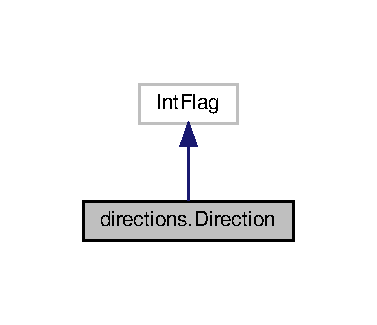
\includegraphics[width=181pt]{classdirections_1_1Direction__inherit__graph}
\end{center}
\end{figure}


Graphe de collaboration de directions.\+Direction\+:\nopagebreak
\begin{figure}[H]
\begin{center}
\leavevmode
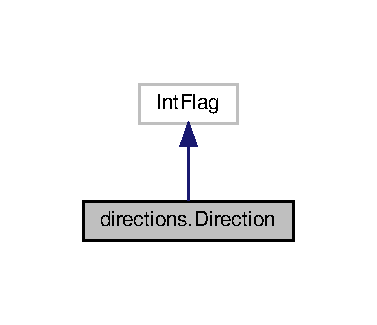
\includegraphics[width=181pt]{classdirections_1_1Direction__coll__graph}
\end{center}
\end{figure}
\subsection*{Fonctions membres publiques}
\begin{DoxyCompactItemize}
\item 
\mbox{\Hypertarget{classdirections_1_1Direction_aba6a03a0ea2b8173c63b7961f12ab28b}\label{classdirections_1_1Direction_aba6a03a0ea2b8173c63b7961f12ab28b}} 
def {\bfseries \+\_\+\+\_\+str\+\_\+\+\_\+} (self)
\item 
\mbox{\Hypertarget{classdirections_1_1Direction_ad3605045e9180a055012bcb7a99df303}\label{classdirections_1_1Direction_ad3605045e9180a055012bcb7a99df303}} 
def {\bfseries from\+\_\+str} (cls, string)
\end{DoxyCompactItemize}
\subsection*{Attributs publics statiques}
\begin{DoxyCompactItemize}
\item 
\mbox{\Hypertarget{classdirections_1_1Direction_a61083067da15f0c0e1a8d8ac9c725d5b}\label{classdirections_1_1Direction_a61083067da15f0c0e1a8d8ac9c725d5b}} 
int {\bfseries N} = 1
\item 
\mbox{\Hypertarget{classdirections_1_1Direction_acff32c8397f7f9a4593149af0b6b58a0}\label{classdirections_1_1Direction_acff32c8397f7f9a4593149af0b6b58a0}} 
int {\bfseries E} = 2
\item 
\mbox{\Hypertarget{classdirections_1_1Direction_a226aeb37b6b75116dc345835a6686f99}\label{classdirections_1_1Direction_a226aeb37b6b75116dc345835a6686f99}} 
int {\bfseries S} = 4
\item 
\mbox{\Hypertarget{classdirections_1_1Direction_aa7d4691007527f96a7545ec36ce6a25c}\label{classdirections_1_1Direction_aa7d4691007527f96a7545ec36ce6a25c}} 
int {\bfseries W} = 8
\end{DoxyCompactItemize}


La documentation de cette classe a été générée à partir du fichier suivant \+:\begin{DoxyCompactItemize}
\item 
directions.\+py\end{DoxyCompactItemize}

\hypertarget{classmain_1_1Exit__window}{}\section{Référence de la classe main.\+Exit\+\_\+window}
\label{classmain_1_1Exit__window}\index{main.\+Exit\+\_\+window@{main.\+Exit\+\_\+window}}


Graphe d\textquotesingle{}héritage de main.\+Exit\+\_\+window\+:
\nopagebreak
\begin{figure}[H]
\begin{center}
\leavevmode
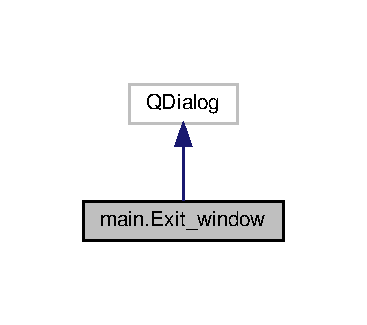
\includegraphics[width=176pt]{classmain_1_1Exit__window__inherit__graph}
\end{center}
\end{figure}


Graphe de collaboration de main.\+Exit\+\_\+window\+:
\nopagebreak
\begin{figure}[H]
\begin{center}
\leavevmode
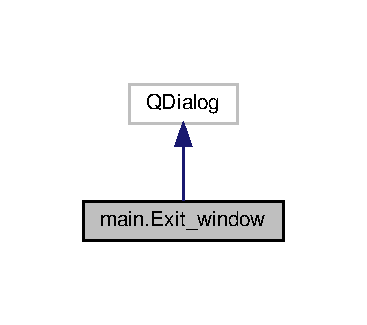
\includegraphics[width=176pt]{classmain_1_1Exit__window__coll__graph}
\end{center}
\end{figure}
\subsection*{Fonctions membres publiques}
\begin{DoxyCompactItemize}
\item 
\mbox{\Hypertarget{classmain_1_1Exit__window_a9f90ad952d59d9cc730182f9e616be8d}\label{classmain_1_1Exit__window_a9f90ad952d59d9cc730182f9e616be8d}} 
def {\bfseries \+\_\+\+\_\+init\+\_\+\+\_\+} (self, number\+\_\+moves)
\item 
\mbox{\Hypertarget{classmain_1_1Exit__window_a87318378bc22e8390da9d0fb55bdc68e}\label{classmain_1_1Exit__window_a87318378bc22e8390da9d0fb55bdc68e}} 
def {\bfseries replay} (self)
\item 
\mbox{\Hypertarget{classmain_1_1Exit__window_a75336f76b626c6295d90ff9f9e58c327}\label{classmain_1_1Exit__window_a75336f76b626c6295d90ff9f9e58c327}} 
def {\bfseries new\+\_\+game} (self)
\item 
\mbox{\Hypertarget{classmain_1_1Exit__window_aedeb6b109d4721ccf4df0dcfc4d4313e}\label{classmain_1_1Exit__window_aedeb6b109d4721ccf4df0dcfc4d4313e}} 
def {\bfseries exit\+\_\+game} (self)
\end{DoxyCompactItemize}
\subsection*{Attributs publics}
\begin{DoxyCompactItemize}
\item 
\mbox{\Hypertarget{classmain_1_1Exit__window_a21b16b6310bf80914b483e2439f4dac3}\label{classmain_1_1Exit__window_a21b16b6310bf80914b483e2439f4dac3}} 
{\bfseries end\+\_\+msg}
\item 
\mbox{\Hypertarget{classmain_1_1Exit__window_ab7058381e75bb04bf887e083aecc3bc3}\label{classmain_1_1Exit__window_ab7058381e75bb04bf887e083aecc3bc3}} 
{\bfseries ret\+Status}
\end{DoxyCompactItemize}


\subsection{Description détaillée}
\begin{DoxyVerb}Fenêtre apparaissant lorsqu'on a gagné. On génère une fonction exit_windows dont le code de retour 1, 2 ou 3 valide le choix :
1 : replay : on remet l'état initial du jeu
2 : new game : on choisit une grille aleatoire
3 : exit : on quitte le jeu.
\end{DoxyVerb}
 

La documentation de cette classe a été générée à partir du fichier suivant \+:\begin{DoxyCompactItemize}
\item 
main.\+py\end{DoxyCompactItemize}

\hypertarget{classgame_1_1Game}{}\section{Référence de la classe game.\+Game}
\label{classgame_1_1Game}\index{game.\+Game@{game.\+Game}}
\subsection*{Fonctions membres publiques}
\begin{DoxyCompactItemize}
\item 
def \hyperlink{classgame_1_1Game_af5743a4c7beabed4dd5dea74a39bbb99}{\+\_\+\+\_\+init\+\_\+\+\_\+} (self, board, robots, goal, record=True)
\item 
\mbox{\Hypertarget{classgame_1_1Game_a2ccf23306726654420eec1a50f67d1cb}\label{classgame_1_1Game_a2ccf23306726654420eec1a50f67d1cb}} 
def {\bfseries add\+\_\+board} (self, board)
\item 
\mbox{\Hypertarget{classgame_1_1Game_a7465d51560b2d485db6ed53907cf1397}\label{classgame_1_1Game_a7465d51560b2d485db6ed53907cf1397}} 
def {\bfseries add\+\_\+goal} (self, goal)
\item 
\mbox{\Hypertarget{classgame_1_1Game_a7e642c0246cea6fa82e92247fa4c3b93}\label{classgame_1_1Game_a7e642c0246cea6fa82e92247fa4c3b93}} 
def {\bfseries add\+\_\+robots} (self, robots)
\item 
def \hyperlink{classgame_1_1Game_aaa2b3e9d8578764bc3eda7ab5841ecbb}{get\+\_\+state} (self)
\item 
def \hyperlink{classgame_1_1Game_a7e87798fb7f81b80c11fcaec17860577}{set\+\_\+state} (self, state)
\item 
def \hyperlink{classgame_1_1Game_a9ae72edd1264e1effe875ec1af8051f9}{state\+\_\+is\+\_\+won} (self, state)
\item 
def \hyperlink{classgame_1_1Game_a0fc708c9734c5a42e3461188580efcd1}{is\+\_\+won} (self)
\item 
def \hyperlink{classgame_1_1Game_a485f03c6330c2bb3284638de65b6cae0}{actions\+\_\+list} (self)
\item 
def \hyperlink{classgame_1_1Game_a2c3428bb9f61284ee0febe00d7850dfa}{do\+\_\+action} (self, action)
\item 
def \hyperlink{classgame_1_1Game_a62f9d3a23be4b342ee35e56cdaf073a3}{do\+\_\+actions} (self, actions)
\item 
def \hyperlink{classgame_1_1Game_a4d05280a8e739b214f50168a7f60c782}{undo} (self)
\item 
def \hyperlink{classgame_1_1Game_a2d8234f8916943384bf5f756b616fe55}{save\+\_\+2\+\_\+json} (self, fp)
\item 
def \hyperlink{classgame_1_1Game_a7c525e5a47b01fb5bed17fe1438c13f5}{save\+\_\+to\+\_\+json} (self, filename)
\end{DoxyCompactItemize}
\subsection*{Fonctions membres publiques statiques}
\begin{DoxyCompactItemize}
\item 
def \hyperlink{classgame_1_1Game_a60b7efdaf394c7f10a249eb7c539afe3}{load\+\_\+from\+\_\+json} (filename)
\end{DoxyCompactItemize}
\subsection*{Attributs publics}
\begin{DoxyCompactItemize}
\item 
\mbox{\Hypertarget{classgame_1_1Game_aebe3d53b7d67e752a35a26d18536c4fa}\label{classgame_1_1Game_aebe3d53b7d67e752a35a26d18536c4fa}} 
{\bfseries board}
\item 
\mbox{\Hypertarget{classgame_1_1Game_a11e55b885ece3eb5e7dfe7772086d55d}\label{classgame_1_1Game_a11e55b885ece3eb5e7dfe7772086d55d}} 
{\bfseries robots}
\item 
\mbox{\Hypertarget{classgame_1_1Game_a74e55df5bbb57b5e22a8b66d6e0d0191}\label{classgame_1_1Game_a74e55df5bbb57b5e22a8b66d6e0d0191}} 
{\bfseries goal}
\item 
\mbox{\Hypertarget{classgame_1_1Game_a5b06cf5a463d3474722aba40c5bb7919}\label{classgame_1_1Game_a5b06cf5a463d3474722aba40c5bb7919}} 
{\bfseries record}
\item 
\mbox{\Hypertarget{classgame_1_1Game_a411615e1fe1f2a51290fa21bd4b8a06a}\label{classgame_1_1Game_a411615e1fe1f2a51290fa21bd4b8a06a}} 
{\bfseries color\+\_\+keys}
\item 
\mbox{\Hypertarget{classgame_1_1Game_a1e1066716b28377232eb2876dfa03dac}\label{classgame_1_1Game_a1e1066716b28377232eb2876dfa03dac}} 
{\bfseries state\+\_\+start}
\item 
\mbox{\Hypertarget{classgame_1_1Game_a48ea4c1038f95e7bedab8cd62e79e76b}\label{classgame_1_1Game_a48ea4c1038f95e7bedab8cd62e79e76b}} 
{\bfseries states\+\_\+list}
\item 
\mbox{\Hypertarget{classgame_1_1Game_a28d186db1f6e43f22a67a9bdd0ae5a0c}\label{classgame_1_1Game_a28d186db1f6e43f22a67a9bdd0ae5a0c}} 
{\bfseries moves\+\_\+list}
\end{DoxyCompactItemize}


\subsection{Documentation des constructeurs et destructeur}
\mbox{\Hypertarget{classgame_1_1Game_af5743a4c7beabed4dd5dea74a39bbb99}\label{classgame_1_1Game_af5743a4c7beabed4dd5dea74a39bbb99}} 
\index{game\+::\+Game@{game\+::\+Game}!\+\_\+\+\_\+init\+\_\+\+\_\+@{\+\_\+\+\_\+init\+\_\+\+\_\+}}
\index{\+\_\+\+\_\+init\+\_\+\+\_\+@{\+\_\+\+\_\+init\+\_\+\+\_\+}!game\+::\+Game@{game\+::\+Game}}
\subsubsection{\texorpdfstring{\+\_\+\+\_\+init\+\_\+\+\_\+()}{\_\_init\_\_()}}
{\footnotesize\ttfamily def game.\+Game.\+\_\+\+\_\+init\+\_\+\+\_\+ (\begin{DoxyParamCaption}\item[{}]{self,  }\item[{}]{board,  }\item[{}]{robots,  }\item[{}]{goal,  }\item[{}]{record = {\ttfamily True} }\end{DoxyParamCaption})}

\begin{DoxyVerb}Constructeur
game = Game(board, robots, goal, record)
Si record est positionné à True, le jeu conserve les différents états dans une pile
ce qui permet de revenir à un état précédent.
\end{DoxyVerb}
 

\subsection{Documentation des fonctions membres}
\mbox{\Hypertarget{classgame_1_1Game_a485f03c6330c2bb3284638de65b6cae0}\label{classgame_1_1Game_a485f03c6330c2bb3284638de65b6cae0}} 
\index{game\+::\+Game@{game\+::\+Game}!actions\+\_\+list@{actions\+\_\+list}}
\index{actions\+\_\+list@{actions\+\_\+list}!game\+::\+Game@{game\+::\+Game}}
\subsubsection{\texorpdfstring{actions\+\_\+list()}{actions\_list()}}
{\footnotesize\ttfamily def game.\+Game.\+actions\+\_\+list (\begin{DoxyParamCaption}\item[{}]{self }\end{DoxyParamCaption})}

\begin{DoxyVerb}Renvoie la liste des actions possibles.
Chaque action est une chaîne de 2 caractères.
Le premier caractère est la couleur du robot, le deuxième est la direction.
Exemple : si game ne comporte qu'un robot rouge
game.actions_list() renvoie ["RN","RE","RS","RW"]
\end{DoxyVerb}
 \mbox{\Hypertarget{classgame_1_1Game_a2c3428bb9f61284ee0febe00d7850dfa}\label{classgame_1_1Game_a2c3428bb9f61284ee0febe00d7850dfa}} 
\index{game\+::\+Game@{game\+::\+Game}!do\+\_\+action@{do\+\_\+action}}
\index{do\+\_\+action@{do\+\_\+action}!game\+::\+Game@{game\+::\+Game}}
\subsubsection{\texorpdfstring{do\+\_\+action()}{do\_action()}}
{\footnotesize\ttfamily def game.\+Game.\+do\+\_\+action (\begin{DoxyParamCaption}\item[{}]{self,  }\item[{}]{action }\end{DoxyParamCaption})}

\begin{DoxyVerb}Demande au jeu d'effectuer l'action décrite par la chaîne de caractères action
Exemple :
    game.do_action("YN") demande au jeu de déplacer le robot Y (yellow) vers le Nord
\end{DoxyVerb}
 \mbox{\Hypertarget{classgame_1_1Game_a62f9d3a23be4b342ee35e56cdaf073a3}\label{classgame_1_1Game_a62f9d3a23be4b342ee35e56cdaf073a3}} 
\index{game\+::\+Game@{game\+::\+Game}!do\+\_\+actions@{do\+\_\+actions}}
\index{do\+\_\+actions@{do\+\_\+actions}!game\+::\+Game@{game\+::\+Game}}
\subsubsection{\texorpdfstring{do\+\_\+actions()}{do\_actions()}}
{\footnotesize\ttfamily def game.\+Game.\+do\+\_\+actions (\begin{DoxyParamCaption}\item[{}]{self,  }\item[{}]{actions }\end{DoxyParamCaption})}

\begin{DoxyVerb}Demande au jeu d'effectuer une liste d'actions les unes à la suite des autres
Renvoie l'état final
\end{DoxyVerb}
 \mbox{\Hypertarget{classgame_1_1Game_aaa2b3e9d8578764bc3eda7ab5841ecbb}\label{classgame_1_1Game_aaa2b3e9d8578764bc3eda7ab5841ecbb}} 
\index{game\+::\+Game@{game\+::\+Game}!get\+\_\+state@{get\+\_\+state}}
\index{get\+\_\+state@{get\+\_\+state}!game\+::\+Game@{game\+::\+Game}}
\subsubsection{\texorpdfstring{get\+\_\+state()}{get\_state()}}
{\footnotesize\ttfamily def game.\+Game.\+get\+\_\+state (\begin{DoxyParamCaption}\item[{}]{self }\end{DoxyParamCaption})}

\begin{DoxyVerb}renvoie l'état du jeu sous forme d'un tuple dcontenant les positions
des robots.
L'ordre des robots dans ce tuple peut être obtenu par l'attribut color_keys
\end{DoxyVerb}
 \mbox{\Hypertarget{classgame_1_1Game_a0fc708c9734c5a42e3461188580efcd1}\label{classgame_1_1Game_a0fc708c9734c5a42e3461188580efcd1}} 
\index{game\+::\+Game@{game\+::\+Game}!is\+\_\+won@{is\+\_\+won}}
\index{is\+\_\+won@{is\+\_\+won}!game\+::\+Game@{game\+::\+Game}}
\subsubsection{\texorpdfstring{is\+\_\+won()}{is\_won()}}
{\footnotesize\ttfamily def game.\+Game.\+is\+\_\+won (\begin{DoxyParamCaption}\item[{}]{self }\end{DoxyParamCaption})}

\begin{DoxyVerb}renvoie True si le jeu est actuellement dans un etat gagnant
\end{DoxyVerb}
 \mbox{\Hypertarget{classgame_1_1Game_a60b7efdaf394c7f10a249eb7c539afe3}\label{classgame_1_1Game_a60b7efdaf394c7f10a249eb7c539afe3}} 
\index{game\+::\+Game@{game\+::\+Game}!load\+\_\+from\+\_\+json@{load\+\_\+from\+\_\+json}}
\index{load\+\_\+from\+\_\+json@{load\+\_\+from\+\_\+json}!game\+::\+Game@{game\+::\+Game}}
\subsubsection{\texorpdfstring{load\+\_\+from\+\_\+json()}{load\_from\_json()}}
{\footnotesize\ttfamily def game.\+Game.\+load\+\_\+from\+\_\+json (\begin{DoxyParamCaption}\item[{}]{filename }\end{DoxyParamCaption})\hspace{0.3cm}{\ttfamily [static]}}

\begin{DoxyVerb}Charge et renvoie un jeu chargé depuis un fichier texte au format json
\end{DoxyVerb}
 \mbox{\Hypertarget{classgame_1_1Game_a2d8234f8916943384bf5f756b616fe55}\label{classgame_1_1Game_a2d8234f8916943384bf5f756b616fe55}} 
\index{game\+::\+Game@{game\+::\+Game}!save\+\_\+2\+\_\+json@{save\+\_\+2\+\_\+json}}
\index{save\+\_\+2\+\_\+json@{save\+\_\+2\+\_\+json}!game\+::\+Game@{game\+::\+Game}}
\subsubsection{\texorpdfstring{save\+\_\+2\+\_\+json()}{save\_2\_json()}}
{\footnotesize\ttfamily def game.\+Game.\+save\+\_\+2\+\_\+json (\begin{DoxyParamCaption}\item[{}]{self,  }\item[{}]{fp }\end{DoxyParamCaption})}

\begin{DoxyVerb}writing data to a text file, using json format
{
"grid" : [ [int, ..., int],
            ...
    [int, ..., int]
    ] ,
"robots" :  {
    "R" : [x , y],

    }
"Goal" : {
    "color" : "R",
    "position" : [x , y]
    }
}
\end{DoxyVerb}
 \mbox{\Hypertarget{classgame_1_1Game_a7c525e5a47b01fb5bed17fe1438c13f5}\label{classgame_1_1Game_a7c525e5a47b01fb5bed17fe1438c13f5}} 
\index{game\+::\+Game@{game\+::\+Game}!save\+\_\+to\+\_\+json@{save\+\_\+to\+\_\+json}}
\index{save\+\_\+to\+\_\+json@{save\+\_\+to\+\_\+json}!game\+::\+Game@{game\+::\+Game}}
\subsubsection{\texorpdfstring{save\+\_\+to\+\_\+json()}{save\_to\_json()}}
{\footnotesize\ttfamily def game.\+Game.\+save\+\_\+to\+\_\+json (\begin{DoxyParamCaption}\item[{}]{self,  }\item[{}]{filename }\end{DoxyParamCaption})}

\begin{DoxyVerb}Ecrit les données de jeu dans un fichier texte, au format json.
Le format est le suivant :
{
"grid" : [ [int, ..., int],
            ...
    [int, ..., int]
    ] ,
"robots" :  {
    "R" : [x, y],
    "Y" : [x, y]
    }
"Goal" : {
    "color" : "R",
    "position" : [x , y]
    }
}
\end{DoxyVerb}
 \mbox{\Hypertarget{classgame_1_1Game_a7e87798fb7f81b80c11fcaec17860577}\label{classgame_1_1Game_a7e87798fb7f81b80c11fcaec17860577}} 
\index{game\+::\+Game@{game\+::\+Game}!set\+\_\+state@{set\+\_\+state}}
\index{set\+\_\+state@{set\+\_\+state}!game\+::\+Game@{game\+::\+Game}}
\subsubsection{\texorpdfstring{set\+\_\+state()}{set\_state()}}
{\footnotesize\ttfamily def game.\+Game.\+set\+\_\+state (\begin{DoxyParamCaption}\item[{}]{self,  }\item[{}]{state }\end{DoxyParamCaption})}

\begin{DoxyVerb}Met le jeu dans l'état décrit par le tuple de positions state
\end{DoxyVerb}
 \mbox{\Hypertarget{classgame_1_1Game_a9ae72edd1264e1effe875ec1af8051f9}\label{classgame_1_1Game_a9ae72edd1264e1effe875ec1af8051f9}} 
\index{game\+::\+Game@{game\+::\+Game}!state\+\_\+is\+\_\+won@{state\+\_\+is\+\_\+won}}
\index{state\+\_\+is\+\_\+won@{state\+\_\+is\+\_\+won}!game\+::\+Game@{game\+::\+Game}}
\subsubsection{\texorpdfstring{state\+\_\+is\+\_\+won()}{state\_is\_won()}}
{\footnotesize\ttfamily def game.\+Game.\+state\+\_\+is\+\_\+won (\begin{DoxyParamCaption}\item[{}]{self,  }\item[{}]{state }\end{DoxyParamCaption})}

\begin{DoxyVerb}renvoie True si state est un état gagnant
\end{DoxyVerb}
 \mbox{\Hypertarget{classgame_1_1Game_a4d05280a8e739b214f50168a7f60c782}\label{classgame_1_1Game_a4d05280a8e739b214f50168a7f60c782}} 
\index{game\+::\+Game@{game\+::\+Game}!undo@{undo}}
\index{undo@{undo}!game\+::\+Game@{game\+::\+Game}}
\subsubsection{\texorpdfstring{undo()}{undo()}}
{\footnotesize\ttfamily def game.\+Game.\+undo (\begin{DoxyParamCaption}\item[{}]{self }\end{DoxyParamCaption})}

\begin{DoxyVerb}Demande au jeu de revenir à l'état précedent
Pour utiliser cette fonctionnalité il faut avoir créé le jeu avec record = True
\end{DoxyVerb}
 

La documentation de cette classe a été générée à partir du fichier suivant \+:\begin{DoxyCompactItemize}
\item 
game.\+py\end{DoxyCompactItemize}

\hypertarget{classgoal_1_1Goal}{}\section{Référence de la classe goal.\+Goal}
\label{classgoal_1_1Goal}\index{goal.\+Goal@{goal.\+Goal}}
\subsection*{Fonctions membres publiques}
\begin{DoxyCompactItemize}
\item 
def \hyperlink{classgoal_1_1Goal_ab9a39523eac5144fe1102e23e94acd5b}{\+\_\+\+\_\+init\+\_\+\+\_\+} (self, color, position)
\item 
def \hyperlink{classgoal_1_1Goal_af125fb03f7d4358fbf776a30da242df1}{\+\_\+\+\_\+str\+\_\+\+\_\+} (self)
\end{DoxyCompactItemize}
\subsection*{Attributs publics}
\begin{DoxyCompactItemize}
\item 
\mbox{\Hypertarget{classgoal_1_1Goal_a54d5132d78565d7996ec4c31c41a0192}\label{classgoal_1_1Goal_a54d5132d78565d7996ec4c31c41a0192}} 
{\bfseries color}
\item 
\mbox{\Hypertarget{classgoal_1_1Goal_a33e1f2b7e55c34c8288aef4f79697d23}\label{classgoal_1_1Goal_a33e1f2b7e55c34c8288aef4f79697d23}} 
{\bfseries position}
\end{DoxyCompactItemize}


\subsection{Documentation des constructeurs et destructeur}
\mbox{\Hypertarget{classgoal_1_1Goal_ab9a39523eac5144fe1102e23e94acd5b}\label{classgoal_1_1Goal_ab9a39523eac5144fe1102e23e94acd5b}} 
\index{goal\+::\+Goal@{goal\+::\+Goal}!\+\_\+\+\_\+init\+\_\+\+\_\+@{\+\_\+\+\_\+init\+\_\+\+\_\+}}
\index{\+\_\+\+\_\+init\+\_\+\+\_\+@{\+\_\+\+\_\+init\+\_\+\+\_\+}!goal\+::\+Goal@{goal\+::\+Goal}}
\subsubsection{\texorpdfstring{\+\_\+\+\_\+init\+\_\+\+\_\+()}{\_\_init\_\_()}}
{\footnotesize\ttfamily def goal.\+Goal.\+\_\+\+\_\+init\+\_\+\+\_\+ (\begin{DoxyParamCaption}\item[{}]{self,  }\item[{}]{color,  }\item[{}]{position }\end{DoxyParamCaption})}

\begin{DoxyVerb}initialisation d'un objet Goal \end{DoxyVerb}
 

\subsection{Documentation des fonctions membres}
\mbox{\Hypertarget{classgoal_1_1Goal_af125fb03f7d4358fbf776a30da242df1}\label{classgoal_1_1Goal_af125fb03f7d4358fbf776a30da242df1}} 
\index{goal\+::\+Goal@{goal\+::\+Goal}!\+\_\+\+\_\+str\+\_\+\+\_\+@{\+\_\+\+\_\+str\+\_\+\+\_\+}}
\index{\+\_\+\+\_\+str\+\_\+\+\_\+@{\+\_\+\+\_\+str\+\_\+\+\_\+}!goal\+::\+Goal@{goal\+::\+Goal}}
\subsubsection{\texorpdfstring{\+\_\+\+\_\+str\+\_\+\+\_\+()}{\_\_str\_\_()}}
{\footnotesize\ttfamily def goal.\+Goal.\+\_\+\+\_\+str\+\_\+\+\_\+ (\begin{DoxyParamCaption}\item[{}]{self }\end{DoxyParamCaption})}

\begin{DoxyVerb}renvoie une chaîne de caractère décrivant l'objectif du jeu 
La chaîne est de la forme :
'"goal" : { "color" : "R",
    "position" : [x,y]
    }
\end{DoxyVerb}
 

La documentation de cette classe a été générée à partir du fichier suivant \+:\begin{DoxyCompactItemize}
\item 
goal.\+py\end{DoxyCompactItemize}

\hypertarget{classmain_1_1Help__window}{}\section{Référence de la classe main.\+Help\+\_\+window}
\label{classmain_1_1Help__window}\index{main.\+Help\+\_\+window@{main.\+Help\+\_\+window}}


Graphe d\textquotesingle{}héritage de main.\+Help\+\_\+window\+:
\nopagebreak
\begin{figure}[H]
\begin{center}
\leavevmode
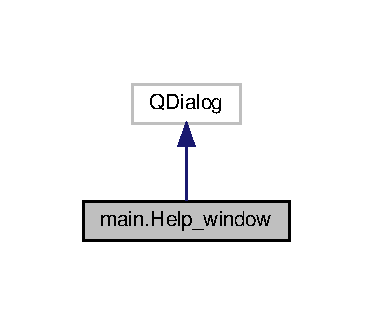
\includegraphics[width=179pt]{classmain_1_1Help__window__inherit__graph}
\end{center}
\end{figure}


Graphe de collaboration de main.\+Help\+\_\+window\+:
\nopagebreak
\begin{figure}[H]
\begin{center}
\leavevmode
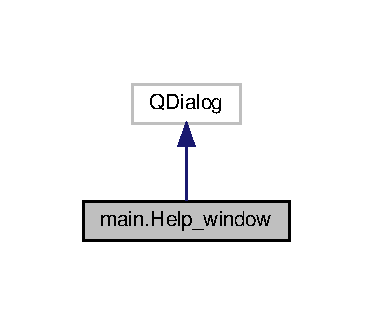
\includegraphics[width=179pt]{classmain_1_1Help__window__coll__graph}
\end{center}
\end{figure}
\subsection*{Fonctions membres publiques}
\begin{DoxyCompactItemize}
\item 
\mbox{\Hypertarget{classmain_1_1Help__window_a1ed494c3053c64389179c2daa132ea8c}\label{classmain_1_1Help__window_a1ed494c3053c64389179c2daa132ea8c}} 
def {\bfseries \+\_\+\+\_\+init\+\_\+\+\_\+} (self)
\end{DoxyCompactItemize}


La documentation de cette classe a été générée à partir du fichier suivant \+:\begin{DoxyCompactItemize}
\item 
main.\+py\end{DoxyCompactItemize}

\hypertarget{classmain_1_1MainWindow}{}\section{Référence de la classe main.\+Main\+Window}
\label{classmain_1_1MainWindow}\index{main.\+Main\+Window@{main.\+Main\+Window}}


Graphe d\textquotesingle{}héritage de main.\+Main\+Window\+:
\nopagebreak
\begin{figure}[H]
\begin{center}
\leavevmode
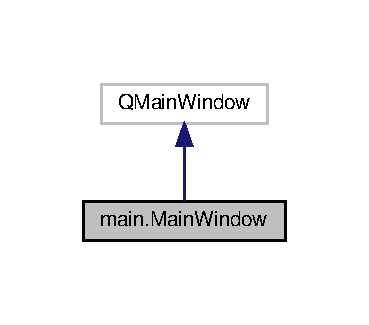
\includegraphics[width=177pt]{classmain_1_1MainWindow__inherit__graph}
\end{center}
\end{figure}


Graphe de collaboration de main.\+Main\+Window\+:
\nopagebreak
\begin{figure}[H]
\begin{center}
\leavevmode
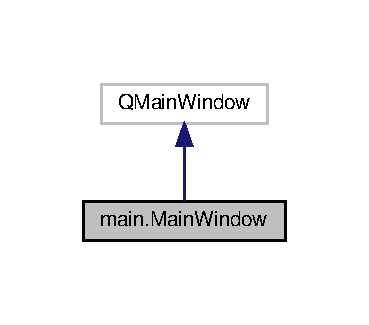
\includegraphics[width=177pt]{classmain_1_1MainWindow__coll__graph}
\end{center}
\end{figure}
\subsection*{Fonctions membres publiques}
\begin{DoxyCompactItemize}
\item 
def \hyperlink{classmain_1_1MainWindow_a1a032331db3e5bbe3267696548ae95df}{\+\_\+\+\_\+init\+\_\+\+\_\+} (self, game)
\item 
def \hyperlink{classmain_1_1MainWindow_ad778ae6b83bc497287aa2f86907a4615}{replay} (self)
\item 
def \hyperlink{classmain_1_1MainWindow_afd6674a5ffab5505719cf020fd430ce0}{help} (self)
\item 
def \hyperlink{classmain_1_1MainWindow_a521027a76aa1c1a13e897137ad43c7d9}{toolbar\+\_\+menus} (self)
\item 
def \hyperlink{classmain_1_1MainWindow_a960159ca187e8bb3a2a53a6ba312331c}{open\+\_\+grid} (self)
\item 
def \hyperlink{classmain_1_1MainWindow_a841e6a28b64e63e03be4fd0073a38ce4}{open\+\_\+game} (self)
\item 
def \hyperlink{classmain_1_1MainWindow_a558ce5d5b1925ec43d49e7acdf5af822}{save\+\_\+grid} (self)
\item 
def \hyperlink{classmain_1_1MainWindow_a208742a5aac99355ae19aee19e9f6419}{save\+\_\+game} (self)
\item 
def \hyperlink{classmain_1_1MainWindow_ad908d5e23984194a3d4dd878489931c4}{print\+\_\+moves\+\_\+list} (self)
\item 
def \hyperlink{classmain_1_1MainWindow_a8c46b65de1e73cd947c826d02d31af4c}{unprint\+\_\+moves\+\_\+list} (self)
\item 
def \hyperlink{classmain_1_1MainWindow_aa7696020f657685831fd5aa212c28e34}{print\+\_\+tip} (self)
\item 
def \hyperlink{classmain_1_1MainWindow_a5ef7f82048e9f0fc50b1f0e1662c9e79}{unprint\+\_\+tip} (self)
\item 
\mbox{\Hypertarget{classmain_1_1MainWindow_a92b541a5faac6214fb37270d19f50038}\label{classmain_1_1MainWindow_a92b541a5faac6214fb37270d19f50038}} 
def {\bfseries choice\+\_\+of\+\_\+grid\+\_\+menu} (self)
\item 
def \hyperlink{classmain_1_1MainWindow_a58e160cf36543e63aa78558a54e9fea1}{choix\+\_\+grille} (self, i)
\item 
\mbox{\Hypertarget{classmain_1_1MainWindow_ac496b3996d4a5bc369742de428f9376b}\label{classmain_1_1MainWindow_ac496b3996d4a5bc369742de428f9376b}} 
def {\bfseries nb\+\_\+robots\+\_\+choice\+\_\+menu} (self)
\item 
def \hyperlink{classmain_1_1MainWindow_a50159f6962a6bd8c7195fe9161b7e009}{choix\+\_\+nb\+\_\+robots} (self, i)
\item 
def \hyperlink{classmain_1_1MainWindow_a53f8ac0e3d2019681c8eff18c541f412}{draw\+\_\+grid} (self)
\item 
\mbox{\Hypertarget{classmain_1_1MainWindow_af920c34bd964662568210e746e9b0f4a}\label{classmain_1_1MainWindow_af920c34bd964662568210e746e9b0f4a}} 
def {\bfseries draw\+\_\+robots\+\_\+and\+\_\+goal} (self)
\item 
\mbox{\Hypertarget{classmain_1_1MainWindow_ae5d6915152ab579f8d85f026f691db90}\label{classmain_1_1MainWindow_ae5d6915152ab579f8d85f026f691db90}} 
def {\bfseries on\+Button\+East\+Click} (self, s)
\item 
\mbox{\Hypertarget{classmain_1_1MainWindow_a086738f56e0bae6b6273fe09110b9e2a}\label{classmain_1_1MainWindow_a086738f56e0bae6b6273fe09110b9e2a}} 
def {\bfseries on\+Button\+West\+Click} (self, s)
\item 
\mbox{\Hypertarget{classmain_1_1MainWindow_a11be49e9d2d28764a9aad869f433dcd4}\label{classmain_1_1MainWindow_a11be49e9d2d28764a9aad869f433dcd4}} 
def {\bfseries on\+Button\+North\+Click} (self, s)
\item 
\mbox{\Hypertarget{classmain_1_1MainWindow_aec9b3412e7a01906698046f97d21b86b}\label{classmain_1_1MainWindow_aec9b3412e7a01906698046f97d21b86b}} 
def {\bfseries on\+Button\+South\+Click} (self, s)
\item 
def \hyperlink{classmain_1_1MainWindow_a61ccbf8b887753b6db3ff19e65e4bc9b}{placer\+\_\+aleatoirement} (self)
\item 
\mbox{\Hypertarget{classmain_1_1MainWindow_a13d3cec7b148ad5e02e08996385bb025}\label{classmain_1_1MainWindow_a13d3cec7b148ad5e02e08996385bb025}} 
def {\bfseries on\+Button\+Red\+Click} (self, s)
\item 
\mbox{\Hypertarget{classmain_1_1MainWindow_a7859745f1e0d3b62232668e14855cf6a}\label{classmain_1_1MainWindow_a7859745f1e0d3b62232668e14855cf6a}} 
def {\bfseries on\+Button\+Green\+Click} (self, s)
\item 
\mbox{\Hypertarget{classmain_1_1MainWindow_a03f83e48e6fc5e884575cd92d417ee34}\label{classmain_1_1MainWindow_a03f83e48e6fc5e884575cd92d417ee34}} 
def {\bfseries on\+Button\+Blue\+Click} (self, s)
\item 
\mbox{\Hypertarget{classmain_1_1MainWindow_abfa9af4e58cc942bd354c0aa1fcb738c}\label{classmain_1_1MainWindow_abfa9af4e58cc942bd354c0aa1fcb738c}} 
def {\bfseries on\+Button\+Yellow\+Click} (self, s)
\item 
def \hyperlink{classmain_1_1MainWindow_a2acd695c824c327fa90308bc2ee511f3}{on\+Button\+Undo\+Click} (self, s)
\item 
def \hyperlink{classmain_1_1MainWindow_a5d1cca4f479efac16adbe9c980368bb3}{solve} (self)
\item 
def \hyperlink{classmain_1_1MainWindow_a26dc40b9b5d9e0327b0f593850746448}{on\+Button\+Tip\+Click} (self, s)
\item 
\mbox{\Hypertarget{classmain_1_1MainWindow_a343f56df8e91b284ad76c72a1b132e7c}\label{classmain_1_1MainWindow_a343f56df8e91b284ad76c72a1b132e7c}} 
def {\bfseries on\+Button\+Solution\+Click} (self, s)
\item 
def \hyperlink{classmain_1_1MainWindow_aa3f0bb9335d7040e1b09e1bd4c9352b8}{game\+\_\+is\+\_\+won} (self)
\end{DoxyCompactItemize}
\subsection*{Attributs publics}
\begin{DoxyCompactItemize}
\item 
\mbox{\Hypertarget{classmain_1_1MainWindow_a218cf92add9b0dfe0654c1bbc8c69206}\label{classmain_1_1MainWindow_a218cf92add9b0dfe0654c1bbc8c69206}} 
{\bfseries game}
\item 
\mbox{\Hypertarget{classmain_1_1MainWindow_a69ff38af7f62102fbf0996afb8f1d600}\label{classmain_1_1MainWindow_a69ff38af7f62102fbf0996afb8f1d600}} 
{\bfseries initial\+\_\+game\+\_\+state}
\item 
\mbox{\Hypertarget{classmain_1_1MainWindow_a505d4ad47ce57e88977a21cd676b5437}\label{classmain_1_1MainWindow_a505d4ad47ce57e88977a21cd676b5437}} 
{\bfseries number\+\_\+moves}
\item 
\mbox{\Hypertarget{classmain_1_1MainWindow_a73b410e7296e8831862de8463b8a5ac7}\label{classmain_1_1MainWindow_a73b410e7296e8831862de8463b8a5ac7}} 
{\bfseries label}
\item 
\mbox{\Hypertarget{classmain_1_1MainWindow_a5513e743525ea6e7fd8e40af818ee2ed}\label{classmain_1_1MainWindow_a5513e743525ea6e7fd8e40af818ee2ed}} 
{\bfseries moves\+\_\+label}
\item 
\mbox{\Hypertarget{classmain_1_1MainWindow_a88ed9245aeaeec4bec2b585e78ac9629}\label{classmain_1_1MainWindow_a88ed9245aeaeec4bec2b585e78ac9629}} 
{\bfseries tip\+\_\+label}
\item 
\mbox{\Hypertarget{classmain_1_1MainWindow_a7c8d9bfed6a783d240b0d667ba184c23}\label{classmain_1_1MainWindow_a7c8d9bfed6a783d240b0d667ba184c23}} 
{\bfseries solution\+\_\+label}
\item 
\mbox{\Hypertarget{classmain_1_1MainWindow_a77421ad8c0efa51641900617a26ff7c3}\label{classmain_1_1MainWindow_a77421ad8c0efa51641900617a26ff7c3}} 
{\bfseries menu}
\item 
\mbox{\Hypertarget{classmain_1_1MainWindow_ac44e7b04f3ca41b523142146661d882d}\label{classmain_1_1MainWindow_ac44e7b04f3ca41b523142146661d882d}} 
{\bfseries file\+\_\+menu}
\item 
\mbox{\Hypertarget{classmain_1_1MainWindow_a3cb629d5307012317ed8b199cc55932f}\label{classmain_1_1MainWindow_a3cb629d5307012317ed8b199cc55932f}} 
{\bfseries help\+\_\+menu}
\item 
\mbox{\Hypertarget{classmain_1_1MainWindow_a4c9516d31dbbd8821bf45f67f637a8f4}\label{classmain_1_1MainWindow_a4c9516d31dbbd8821bf45f67f637a8f4}} 
{\bfseries size\+\_\+fenetre}
\item 
\mbox{\Hypertarget{classmain_1_1MainWindow_a5f6accc2264e83bc9b92047e2a79072e}\label{classmain_1_1MainWindow_a5f6accc2264e83bc9b92047e2a79072e}} 
{\bfseries selected\+\_\+robot}
\item 
\mbox{\Hypertarget{classmain_1_1MainWindow_a98485c685a1dfe53b3cc2759f56b2588}\label{classmain_1_1MainWindow_a98485c685a1dfe53b3cc2759f56b2588}} 
{\bfseries help\+\_\+windows}
\item 
\mbox{\Hypertarget{classmain_1_1MainWindow_a65dd0e10162c0c2bcb694480572b6ba7}\label{classmain_1_1MainWindow_a65dd0e10162c0c2bcb694480572b6ba7}} 
{\bfseries group}
\item 
\mbox{\Hypertarget{classmain_1_1MainWindow_a380fc7d29cd899d05a0dea12625bf945}\label{classmain_1_1MainWindow_a380fc7d29cd899d05a0dea12625bf945}} 
{\bfseries grid\+\_\+choice}
\item 
\mbox{\Hypertarget{classmain_1_1MainWindow_abb338ff5b88588c54bfd5242ebc693e9}\label{classmain_1_1MainWindow_abb338ff5b88588c54bfd5242ebc693e9}} 
{\bfseries nb\+\_\+robots\+\_\+choice}
\item 
\mbox{\Hypertarget{classmain_1_1MainWindow_a87cc9e24804a2929e0e7691460ea0b9d}\label{classmain_1_1MainWindow_a87cc9e24804a2929e0e7691460ea0b9d}} 
{\bfseries nb\+\_\+robots}
\item 
\mbox{\Hypertarget{classmain_1_1MainWindow_a5849cdc0d3b9ff8a89f32ba8899636ab}\label{classmain_1_1MainWindow_a5849cdc0d3b9ff8a89f32ba8899636ab}} 
{\bfseries placement\+\_\+aleatoire}
\item 
\mbox{\Hypertarget{classmain_1_1MainWindow_a1b211d8a7224e262635eef8c71fb7549}\label{classmain_1_1MainWindow_a1b211d8a7224e262635eef8c71fb7549}} 
{\bfseries tip\+\_\+game}
\item 
\mbox{\Hypertarget{classmain_1_1MainWindow_af722734aedc44e39b790634a32a715bc}\label{classmain_1_1MainWindow_af722734aedc44e39b790634a32a715bc}} 
{\bfseries tip}
\item 
\mbox{\Hypertarget{classmain_1_1MainWindow_aa52848bbd0e0c9f9820e5a15ae80d567}\label{classmain_1_1MainWindow_aa52848bbd0e0c9f9820e5a15ae80d567}} 
{\bfseries solution}
\item 
\mbox{\Hypertarget{classmain_1_1MainWindow_a327eb8635518582db97862f4276319d4}\label{classmain_1_1MainWindow_a327eb8635518582db97862f4276319d4}} 
{\bfseries exit\+\_\+windows}
\end{DoxyCompactItemize}
\subsection*{Attributs publics statiques}
\begin{DoxyCompactItemize}
\item 
\mbox{\Hypertarget{classmain_1_1MainWindow_a15e75bbd8a9684532615c7f5e926dd9e}\label{classmain_1_1MainWindow_a15e75bbd8a9684532615c7f5e926dd9e}} 
int {\bfseries D\+I\+M\+E\+N\+S\+I\+ON} = 560
\item 
\mbox{\Hypertarget{classmain_1_1MainWindow_a669de576e29e0cba21864576b54cf07a}\label{classmain_1_1MainWindow_a669de576e29e0cba21864576b54cf07a}} 
bool {\bfseries placement\+\_\+aleatoire} = True
\item 
\mbox{\Hypertarget{classmain_1_1MainWindow_a1c9eeb17286bfe6ca3dd736a8242fbe5}\label{classmain_1_1MainWindow_a1c9eeb17286bfe6ca3dd736a8242fbe5}} 
int {\bfseries nb\+\_\+robots} = 0
\end{DoxyCompactItemize}


\subsection{Documentation des constructeurs et destructeur}
\mbox{\Hypertarget{classmain_1_1MainWindow_a1a032331db3e5bbe3267696548ae95df}\label{classmain_1_1MainWindow_a1a032331db3e5bbe3267696548ae95df}} 
\index{main\+::\+Main\+Window@{main\+::\+Main\+Window}!\+\_\+\+\_\+init\+\_\+\+\_\+@{\+\_\+\+\_\+init\+\_\+\+\_\+}}
\index{\+\_\+\+\_\+init\+\_\+\+\_\+@{\+\_\+\+\_\+init\+\_\+\+\_\+}!main\+::\+Main\+Window@{main\+::\+Main\+Window}}
\subsubsection{\texorpdfstring{\+\_\+\+\_\+init\+\_\+\+\_\+()}{\_\_init\_\_()}}
{\footnotesize\ttfamily def main.\+Main\+Window.\+\_\+\+\_\+init\+\_\+\+\_\+ (\begin{DoxyParamCaption}\item[{}]{self,  }\item[{}]{game }\end{DoxyParamCaption})}

\begin{DoxyVerb}La fenêtre principale est initialisée avec l'organisation suivante :

+--------------------------------------------------------------------------+
|              self.menu = self.menuBar()                                  |
|                                                                          |
+--------------------------------------------------------------------------+
|       toolbar = QToolBar()  (déplacement/sélection des robots,           |
|                     boutons annuler, indice et solution)                 |
+------------------------layout0 = QHBoxLayout()---------------------------+
|    layout2 = QHBoxLayout()                  +      moves_label           |
| l                    +                      |                            |
| a  grid_choice       |  nb_robots_choice    |     (affichage des         |
+-y--------------------+----------------------+  L                         |
| o                                           |  a  mouvements effectués)  |
| u                                           |  y                         |
| t                                           +--o-------------------------+
| =          label = QLabel()                 |  u                         |
| Q                                           |  t     tip_label           |
| V          contient la grille de jeu        |  3                         |
| B                                           |      (Affichage de l'indice|
| o                                           |  =                         |
| x                                           |      si demandé)           |
| L                                           |  Q                         |
| a                                           +--V+------------------------+
| y                                           |  B     solution_label      |
| o                                           |  o                         |
| u                                           |  x   (Affichage de la      |
| t                                           |                            |
|                                             |      solution si demandée) |
+---------------------------------------------+----------------------------+\end{DoxyVerb}
 

\subsection{Documentation des fonctions membres}
\mbox{\Hypertarget{classmain_1_1MainWindow_a58e160cf36543e63aa78558a54e9fea1}\label{classmain_1_1MainWindow_a58e160cf36543e63aa78558a54e9fea1}} 
\index{main\+::\+Main\+Window@{main\+::\+Main\+Window}!choix\+\_\+grille@{choix\+\_\+grille}}
\index{choix\+\_\+grille@{choix\+\_\+grille}!main\+::\+Main\+Window@{main\+::\+Main\+Window}}
\subsubsection{\texorpdfstring{choix\+\_\+grille()}{choix\_grille()}}
{\footnotesize\ttfamily def main.\+Main\+Window.\+choix\+\_\+grille (\begin{DoxyParamCaption}\item[{}]{self,  }\item[{}]{i }\end{DoxyParamCaption})}

\begin{DoxyVerb}Lors du choix d'une nouvelle grille, le jeu est réinitialisé et redessiné, les robots et l'objectif sont masqués.
\end{DoxyVerb}
 \mbox{\Hypertarget{classmain_1_1MainWindow_a50159f6962a6bd8c7195fe9161b7e009}\label{classmain_1_1MainWindow_a50159f6962a6bd8c7195fe9161b7e009}} 
\index{main\+::\+Main\+Window@{main\+::\+Main\+Window}!choix\+\_\+nb\+\_\+robots@{choix\+\_\+nb\+\_\+robots}}
\index{choix\+\_\+nb\+\_\+robots@{choix\+\_\+nb\+\_\+robots}!main\+::\+Main\+Window@{main\+::\+Main\+Window}}
\subsubsection{\texorpdfstring{choix\+\_\+nb\+\_\+robots()}{choix\_nb\_robots()}}
{\footnotesize\ttfamily def main.\+Main\+Window.\+choix\+\_\+nb\+\_\+robots (\begin{DoxyParamCaption}\item[{}]{self,  }\item[{}]{i }\end{DoxyParamCaption})}

\begin{DoxyVerb}Les robots et l'objectif sont placés aléatoirement. L'extension
\end{DoxyVerb}
 \mbox{\Hypertarget{classmain_1_1MainWindow_a53f8ac0e3d2019681c8eff18c541f412}\label{classmain_1_1MainWindow_a53f8ac0e3d2019681c8eff18c541f412}} 
\index{main\+::\+Main\+Window@{main\+::\+Main\+Window}!draw\+\_\+grid@{draw\+\_\+grid}}
\index{draw\+\_\+grid@{draw\+\_\+grid}!main\+::\+Main\+Window@{main\+::\+Main\+Window}}
\subsubsection{\texorpdfstring{draw\+\_\+grid()}{draw\_grid()}}
{\footnotesize\ttfamily def main.\+Main\+Window.\+draw\+\_\+grid (\begin{DoxyParamCaption}\item[{}]{self }\end{DoxyParamCaption})}

\begin{DoxyVerb}Dessine la grille de jeu en juxtaposant les images contenant chaque case. Chaque image est redimensionnée et ajustée à la taille de la grille.
\end{DoxyVerb}
 \mbox{\Hypertarget{classmain_1_1MainWindow_aa3f0bb9335d7040e1b09e1bd4c9352b8}\label{classmain_1_1MainWindow_aa3f0bb9335d7040e1b09e1bd4c9352b8}} 
\index{main\+::\+Main\+Window@{main\+::\+Main\+Window}!game\+\_\+is\+\_\+won@{game\+\_\+is\+\_\+won}}
\index{game\+\_\+is\+\_\+won@{game\+\_\+is\+\_\+won}!main\+::\+Main\+Window@{main\+::\+Main\+Window}}
\subsubsection{\texorpdfstring{game\+\_\+is\+\_\+won()}{game\_is\_won()}}
{\footnotesize\ttfamily def main.\+Main\+Window.\+game\+\_\+is\+\_\+won (\begin{DoxyParamCaption}\item[{}]{self }\end{DoxyParamCaption})}

\begin{DoxyVerb}Fonction lancée quand l'objectif est atteint. On génère une fonction exit_windows dont le code de retour 1, 2 ou 3 valide le choix :
1 : replay : on remet l'état initial du jeu
2 : new game : on choisit une grille aleatoire
3 : exit : on quitte le jeu.
\end{DoxyVerb}
 \mbox{\Hypertarget{classmain_1_1MainWindow_afd6674a5ffab5505719cf020fd430ce0}\label{classmain_1_1MainWindow_afd6674a5ffab5505719cf020fd430ce0}} 
\index{main\+::\+Main\+Window@{main\+::\+Main\+Window}!help@{help}}
\index{help@{help}!main\+::\+Main\+Window@{main\+::\+Main\+Window}}
\subsubsection{\texorpdfstring{help()}{help()}}
{\footnotesize\ttfamily def main.\+Main\+Window.\+help (\begin{DoxyParamCaption}\item[{}]{self }\end{DoxyParamCaption})}

\begin{DoxyVerb}Ouvre une fenêtre d'aide\end{DoxyVerb}
 \mbox{\Hypertarget{classmain_1_1MainWindow_a26dc40b9b5d9e0327b0f593850746448}\label{classmain_1_1MainWindow_a26dc40b9b5d9e0327b0f593850746448}} 
\index{main\+::\+Main\+Window@{main\+::\+Main\+Window}!on\+Button\+Tip\+Click@{on\+Button\+Tip\+Click}}
\index{on\+Button\+Tip\+Click@{on\+Button\+Tip\+Click}!main\+::\+Main\+Window@{main\+::\+Main\+Window}}
\subsubsection{\texorpdfstring{on\+Button\+Tip\+Click()}{onButtonTipClick()}}
{\footnotesize\ttfamily def main.\+Main\+Window.\+on\+Button\+Tip\+Click (\begin{DoxyParamCaption}\item[{}]{self,  }\item[{}]{s }\end{DoxyParamCaption})}

\begin{DoxyVerb}La solution renvoyée par le solveur est de la forme (True/False, liste d'actions à effectuer).
On récupère ici la première action.\end{DoxyVerb}
 \mbox{\Hypertarget{classmain_1_1MainWindow_a2acd695c824c327fa90308bc2ee511f3}\label{classmain_1_1MainWindow_a2acd695c824c327fa90308bc2ee511f3}} 
\index{main\+::\+Main\+Window@{main\+::\+Main\+Window}!on\+Button\+Undo\+Click@{on\+Button\+Undo\+Click}}
\index{on\+Button\+Undo\+Click@{on\+Button\+Undo\+Click}!main\+::\+Main\+Window@{main\+::\+Main\+Window}}
\subsubsection{\texorpdfstring{on\+Button\+Undo\+Click()}{onButtonUndoClick()}}
{\footnotesize\ttfamily def main.\+Main\+Window.\+on\+Button\+Undo\+Click (\begin{DoxyParamCaption}\item[{}]{self,  }\item[{}]{s }\end{DoxyParamCaption})}

\begin{DoxyVerb}Annule le dernier coup effectué \end{DoxyVerb}
 \mbox{\Hypertarget{classmain_1_1MainWindow_a841e6a28b64e63e03be4fd0073a38ce4}\label{classmain_1_1MainWindow_a841e6a28b64e63e03be4fd0073a38ce4}} 
\index{main\+::\+Main\+Window@{main\+::\+Main\+Window}!open\+\_\+game@{open\+\_\+game}}
\index{open\+\_\+game@{open\+\_\+game}!main\+::\+Main\+Window@{main\+::\+Main\+Window}}
\subsubsection{\texorpdfstring{open\+\_\+game()}{open\_game()}}
{\footnotesize\ttfamily def main.\+Main\+Window.\+open\+\_\+game (\begin{DoxyParamCaption}\item[{}]{self }\end{DoxyParamCaption})}

\begin{DoxyVerb}Ouvre une boîte de dialogue permettant de charger un jeu existant sur le disque dur\end{DoxyVerb}
 \mbox{\Hypertarget{classmain_1_1MainWindow_a960159ca187e8bb3a2a53a6ba312331c}\label{classmain_1_1MainWindow_a960159ca187e8bb3a2a53a6ba312331c}} 
\index{main\+::\+Main\+Window@{main\+::\+Main\+Window}!open\+\_\+grid@{open\+\_\+grid}}
\index{open\+\_\+grid@{open\+\_\+grid}!main\+::\+Main\+Window@{main\+::\+Main\+Window}}
\subsubsection{\texorpdfstring{open\+\_\+grid()}{open\_grid()}}
{\footnotesize\ttfamily def main.\+Main\+Window.\+open\+\_\+grid (\begin{DoxyParamCaption}\item[{}]{self }\end{DoxyParamCaption})}

\begin{DoxyVerb}Ouvre une boîte de dialogue permettant de charger une grille existante sur le disque dur\end{DoxyVerb}
 \mbox{\Hypertarget{classmain_1_1MainWindow_a61ccbf8b887753b6db3ff19e65e4bc9b}\label{classmain_1_1MainWindow_a61ccbf8b887753b6db3ff19e65e4bc9b}} 
\index{main\+::\+Main\+Window@{main\+::\+Main\+Window}!placer\+\_\+aleatoirement@{placer\+\_\+aleatoirement}}
\index{placer\+\_\+aleatoirement@{placer\+\_\+aleatoirement}!main\+::\+Main\+Window@{main\+::\+Main\+Window}}
\subsubsection{\texorpdfstring{placer\+\_\+aleatoirement()}{placer\_aleatoirement()}}
{\footnotesize\ttfamily def main.\+Main\+Window.\+placer\+\_\+aleatoirement (\begin{DoxyParamCaption}\item[{}]{self }\end{DoxyParamCaption})}

\begin{DoxyVerb}inverse la sélection de la checkBox \end{DoxyVerb}
 \mbox{\Hypertarget{classmain_1_1MainWindow_ad908d5e23984194a3d4dd878489931c4}\label{classmain_1_1MainWindow_ad908d5e23984194a3d4dd878489931c4}} 
\index{main\+::\+Main\+Window@{main\+::\+Main\+Window}!print\+\_\+moves\+\_\+list@{print\+\_\+moves\+\_\+list}}
\index{print\+\_\+moves\+\_\+list@{print\+\_\+moves\+\_\+list}!main\+::\+Main\+Window@{main\+::\+Main\+Window}}
\subsubsection{\texorpdfstring{print\+\_\+moves\+\_\+list()}{print\_moves\_list()}}
{\footnotesize\ttfamily def main.\+Main\+Window.\+print\+\_\+moves\+\_\+list (\begin{DoxyParamCaption}\item[{}]{self }\end{DoxyParamCaption})}

\begin{DoxyVerb}Affichage de la liste des mouvements effectués dans le label "moves_label" \end{DoxyVerb}
 \mbox{\Hypertarget{classmain_1_1MainWindow_aa7696020f657685831fd5aa212c28e34}\label{classmain_1_1MainWindow_aa7696020f657685831fd5aa212c28e34}} 
\index{main\+::\+Main\+Window@{main\+::\+Main\+Window}!print\+\_\+tip@{print\+\_\+tip}}
\index{print\+\_\+tip@{print\+\_\+tip}!main\+::\+Main\+Window@{main\+::\+Main\+Window}}
\subsubsection{\texorpdfstring{print\+\_\+tip()}{print\_tip()}}
{\footnotesize\ttfamily def main.\+Main\+Window.\+print\+\_\+tip (\begin{DoxyParamCaption}\item[{}]{self }\end{DoxyParamCaption})}

\begin{DoxyVerb}Affichage du conseil généré par le solveur  dans le label "tip_label" \end{DoxyVerb}
 \mbox{\Hypertarget{classmain_1_1MainWindow_ad778ae6b83bc497287aa2f86907a4615}\label{classmain_1_1MainWindow_ad778ae6b83bc497287aa2f86907a4615}} 
\index{main\+::\+Main\+Window@{main\+::\+Main\+Window}!replay@{replay}}
\index{replay@{replay}!main\+::\+Main\+Window@{main\+::\+Main\+Window}}
\subsubsection{\texorpdfstring{replay()}{replay()}}
{\footnotesize\ttfamily def main.\+Main\+Window.\+replay (\begin{DoxyParamCaption}\item[{}]{self }\end{DoxyParamCaption})}

\begin{DoxyVerb}on remet l'état initial du jeu \end{DoxyVerb}
 \mbox{\Hypertarget{classmain_1_1MainWindow_a208742a5aac99355ae19aee19e9f6419}\label{classmain_1_1MainWindow_a208742a5aac99355ae19aee19e9f6419}} 
\index{main\+::\+Main\+Window@{main\+::\+Main\+Window}!save\+\_\+game@{save\+\_\+game}}
\index{save\+\_\+game@{save\+\_\+game}!main\+::\+Main\+Window@{main\+::\+Main\+Window}}
\subsubsection{\texorpdfstring{save\+\_\+game()}{save\_game()}}
{\footnotesize\ttfamily def main.\+Main\+Window.\+save\+\_\+game (\begin{DoxyParamCaption}\item[{}]{self }\end{DoxyParamCaption})}

\begin{DoxyVerb}Ouvre une boîte de dialogue permettant d'enregistrer le jeu actuel sur le disque dur
    Si le joueur entre ou sélectionne un nom de fichier, le eju est sauvegardé dans ce fichier\end{DoxyVerb}
 \mbox{\Hypertarget{classmain_1_1MainWindow_a558ce5d5b1925ec43d49e7acdf5af822}\label{classmain_1_1MainWindow_a558ce5d5b1925ec43d49e7acdf5af822}} 
\index{main\+::\+Main\+Window@{main\+::\+Main\+Window}!save\+\_\+grid@{save\+\_\+grid}}
\index{save\+\_\+grid@{save\+\_\+grid}!main\+::\+Main\+Window@{main\+::\+Main\+Window}}
\subsubsection{\texorpdfstring{save\+\_\+grid()}{save\_grid()}}
{\footnotesize\ttfamily def main.\+Main\+Window.\+save\+\_\+grid (\begin{DoxyParamCaption}\item[{}]{self }\end{DoxyParamCaption})}

\begin{DoxyVerb}Ouvre une boîte de dialogue permettant d'enregistrer la grille affichée sur le disque dur\end{DoxyVerb}
 \mbox{\Hypertarget{classmain_1_1MainWindow_a5d1cca4f479efac16adbe9c980368bb3}\label{classmain_1_1MainWindow_a5d1cca4f479efac16adbe9c980368bb3}} 
\index{main\+::\+Main\+Window@{main\+::\+Main\+Window}!solve@{solve}}
\index{solve@{solve}!main\+::\+Main\+Window@{main\+::\+Main\+Window}}
\subsubsection{\texorpdfstring{solve()}{solve()}}
{\footnotesize\ttfamily def main.\+Main\+Window.\+solve (\begin{DoxyParamCaption}\item[{}]{self }\end{DoxyParamCaption})}

\begin{DoxyVerb}tip_game contient une copie du jeu courant, pour l'utiliser par le solveur\end{DoxyVerb}
 \mbox{\Hypertarget{classmain_1_1MainWindow_a521027a76aa1c1a13e897137ad43c7d9}\label{classmain_1_1MainWindow_a521027a76aa1c1a13e897137ad43c7d9}} 
\index{main\+::\+Main\+Window@{main\+::\+Main\+Window}!toolbar\+\_\+menus@{toolbar\+\_\+menus}}
\index{toolbar\+\_\+menus@{toolbar\+\_\+menus}!main\+::\+Main\+Window@{main\+::\+Main\+Window}}
\subsubsection{\texorpdfstring{toolbar\+\_\+menus()}{toolbar\_menus()}}
{\footnotesize\ttfamily def main.\+Main\+Window.\+toolbar\+\_\+menus (\begin{DoxyParamCaption}\item[{}]{self }\end{DoxyParamCaption})}

\begin{DoxyVerb}Affiche la barre d'icônes permettant de diriger les robots et de les sélectionner\end{DoxyVerb}
 \mbox{\Hypertarget{classmain_1_1MainWindow_a8c46b65de1e73cd947c826d02d31af4c}\label{classmain_1_1MainWindow_a8c46b65de1e73cd947c826d02d31af4c}} 
\index{main\+::\+Main\+Window@{main\+::\+Main\+Window}!unprint\+\_\+moves\+\_\+list@{unprint\+\_\+moves\+\_\+list}}
\index{unprint\+\_\+moves\+\_\+list@{unprint\+\_\+moves\+\_\+list}!main\+::\+Main\+Window@{main\+::\+Main\+Window}}
\subsubsection{\texorpdfstring{unprint\+\_\+moves\+\_\+list()}{unprint\_moves\_list()}}
{\footnotesize\ttfamily def main.\+Main\+Window.\+unprint\+\_\+moves\+\_\+list (\begin{DoxyParamCaption}\item[{}]{self }\end{DoxyParamCaption})}

\begin{DoxyVerb}réinitialisation du label "moves_label" pour cacher la liste des mouvements effectués. \end{DoxyVerb}
 \mbox{\Hypertarget{classmain_1_1MainWindow_a5ef7f82048e9f0fc50b1f0e1662c9e79}\label{classmain_1_1MainWindow_a5ef7f82048e9f0fc50b1f0e1662c9e79}} 
\index{main\+::\+Main\+Window@{main\+::\+Main\+Window}!unprint\+\_\+tip@{unprint\+\_\+tip}}
\index{unprint\+\_\+tip@{unprint\+\_\+tip}!main\+::\+Main\+Window@{main\+::\+Main\+Window}}
\subsubsection{\texorpdfstring{unprint\+\_\+tip()}{unprint\_tip()}}
{\footnotesize\ttfamily def main.\+Main\+Window.\+unprint\+\_\+tip (\begin{DoxyParamCaption}\item[{}]{self }\end{DoxyParamCaption})}

\begin{DoxyVerb}réinitialisation du label "tip_label" pour cacher le conseil généré par le solveur. \end{DoxyVerb}
 

La documentation de cette classe a été générée à partir du fichier suivant \+:\begin{DoxyCompactItemize}
\item 
main.\+py\end{DoxyCompactItemize}

\hypertarget{classgrid__visualiseur_1_1MainWindow}{}\section{Référence de la classe grid\+\_\+visualiseur.\+Main\+Window}
\label{classgrid__visualiseur_1_1MainWindow}\index{grid\+\_\+visualiseur.\+Main\+Window@{grid\+\_\+visualiseur.\+Main\+Window}}


Graphe d\textquotesingle{}héritage de grid\+\_\+visualiseur.\+Main\+Window\+:\nopagebreak
\begin{figure}[H]
\begin{center}
\leavevmode
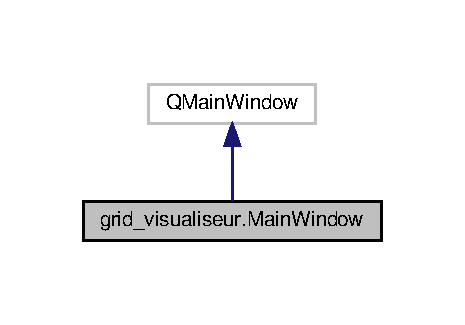
\includegraphics[width=223pt]{classgrid__visualiseur_1_1MainWindow__inherit__graph}
\end{center}
\end{figure}


Graphe de collaboration de grid\+\_\+visualiseur.\+Main\+Window\+:\nopagebreak
\begin{figure}[H]
\begin{center}
\leavevmode
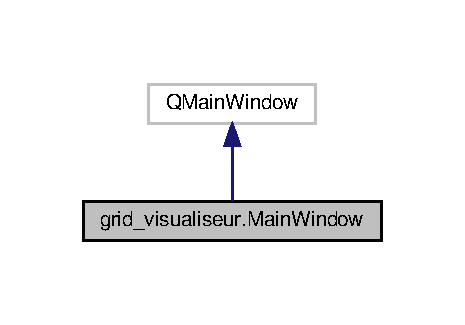
\includegraphics[width=223pt]{classgrid__visualiseur_1_1MainWindow__coll__graph}
\end{center}
\end{figure}
\subsection*{Fonctions membres publiques}
\begin{DoxyCompactItemize}
\item 
def \hyperlink{classgrid__visualiseur_1_1MainWindow_aa58b1a902fbbe5e3ceda337c7ef87658}{\+\_\+\+\_\+init\+\_\+\+\_\+} (self)
\item 
def \hyperlink{classgrid__visualiseur_1_1MainWindow_a4c84e902c352f90578745c1d5112e373}{create\+\_\+menu} (self)
\item 
def \hyperlink{classgrid__visualiseur_1_1MainWindow_a6d4f89a1640755a326a358026815ca66}{open\+\_\+grid} (self)
\item 
def \hyperlink{classgrid__visualiseur_1_1MainWindow_a4915c6cc9059cb6949bc8d1e997e1af1}{draw\+\_\+\+Board} (self, board)
\end{DoxyCompactItemize}
\subsection*{Attributs publics}
\begin{DoxyCompactItemize}
\item 
\mbox{\Hypertarget{classgrid__visualiseur_1_1MainWindow_a1f610c2428199203787c063b39ce3c3e}\label{classgrid__visualiseur_1_1MainWindow_a1f610c2428199203787c063b39ce3c3e}} 
{\bfseries label}
\end{DoxyCompactItemize}


\subsection{Documentation des constructeurs et destructeur}
\mbox{\Hypertarget{classgrid__visualiseur_1_1MainWindow_aa58b1a902fbbe5e3ceda337c7ef87658}\label{classgrid__visualiseur_1_1MainWindow_aa58b1a902fbbe5e3ceda337c7ef87658}} 
\index{grid\+\_\+visualiseur\+::\+Main\+Window@{grid\+\_\+visualiseur\+::\+Main\+Window}!\+\_\+\+\_\+init\+\_\+\+\_\+@{\+\_\+\+\_\+init\+\_\+\+\_\+}}
\index{\+\_\+\+\_\+init\+\_\+\+\_\+@{\+\_\+\+\_\+init\+\_\+\+\_\+}!grid\+\_\+visualiseur\+::\+Main\+Window@{grid\+\_\+visualiseur\+::\+Main\+Window}}
\subsubsection{\texorpdfstring{\+\_\+\+\_\+init\+\_\+\+\_\+()}{\_\_init\_\_()}}
{\footnotesize\ttfamily def grid\+\_\+visualiseur.\+Main\+Window.\+\_\+\+\_\+init\+\_\+\+\_\+ (\begin{DoxyParamCaption}\item[{}]{self }\end{DoxyParamCaption})}

\begin{DoxyVerb}initialisation de la fenêtre du visualiseur \end{DoxyVerb}
 

\subsection{Documentation des fonctions membres}
\mbox{\Hypertarget{classgrid__visualiseur_1_1MainWindow_a4c84e902c352f90578745c1d5112e373}\label{classgrid__visualiseur_1_1MainWindow_a4c84e902c352f90578745c1d5112e373}} 
\index{grid\+\_\+visualiseur\+::\+Main\+Window@{grid\+\_\+visualiseur\+::\+Main\+Window}!create\+\_\+menu@{create\+\_\+menu}}
\index{create\+\_\+menu@{create\+\_\+menu}!grid\+\_\+visualiseur\+::\+Main\+Window@{grid\+\_\+visualiseur\+::\+Main\+Window}}
\subsubsection{\texorpdfstring{create\+\_\+menu()}{create\_menu()}}
{\footnotesize\ttfamily def grid\+\_\+visualiseur.\+Main\+Window.\+create\+\_\+menu (\begin{DoxyParamCaption}\item[{}]{self }\end{DoxyParamCaption})}

\begin{DoxyVerb}création du menu "Fichier" comportant la commande Open \end{DoxyVerb}
 \mbox{\Hypertarget{classgrid__visualiseur_1_1MainWindow_a4915c6cc9059cb6949bc8d1e997e1af1}\label{classgrid__visualiseur_1_1MainWindow_a4915c6cc9059cb6949bc8d1e997e1af1}} 
\index{grid\+\_\+visualiseur\+::\+Main\+Window@{grid\+\_\+visualiseur\+::\+Main\+Window}!draw\+\_\+\+Board@{draw\+\_\+\+Board}}
\index{draw\+\_\+\+Board@{draw\+\_\+\+Board}!grid\+\_\+visualiseur\+::\+Main\+Window@{grid\+\_\+visualiseur\+::\+Main\+Window}}
\subsubsection{\texorpdfstring{draw\+\_\+\+Board()}{draw\_Board()}}
{\footnotesize\ttfamily def grid\+\_\+visualiseur.\+Main\+Window.\+draw\+\_\+\+Board (\begin{DoxyParamCaption}\item[{}]{self,  }\item[{}]{board }\end{DoxyParamCaption})}

\begin{DoxyVerb}dessine la grille dans objet Pixmap \end{DoxyVerb}
 \mbox{\Hypertarget{classgrid__visualiseur_1_1MainWindow_a6d4f89a1640755a326a358026815ca66}\label{classgrid__visualiseur_1_1MainWindow_a6d4f89a1640755a326a358026815ca66}} 
\index{grid\+\_\+visualiseur\+::\+Main\+Window@{grid\+\_\+visualiseur\+::\+Main\+Window}!open\+\_\+grid@{open\+\_\+grid}}
\index{open\+\_\+grid@{open\+\_\+grid}!grid\+\_\+visualiseur\+::\+Main\+Window@{grid\+\_\+visualiseur\+::\+Main\+Window}}
\subsubsection{\texorpdfstring{open\+\_\+grid()}{open\_grid()}}
{\footnotesize\ttfamily def grid\+\_\+visualiseur.\+Main\+Window.\+open\+\_\+grid (\begin{DoxyParamCaption}\item[{}]{self }\end{DoxyParamCaption})}

\begin{DoxyVerb}affiche un dialogue pour l'ouverture d'un fichier \end{DoxyVerb}
 

La documentation de cette classe a été générée à partir du fichier suivant \+:\begin{DoxyCompactItemize}
\item 
grid\+\_\+visualiseur.\+py\end{DoxyCompactItemize}

\hypertarget{classgrid__visualiseur_1_1MyPainter}{}\section{Référence de la classe grid\+\_\+visualiseur.\+My\+Painter}
\label{classgrid__visualiseur_1_1MyPainter}\index{grid\+\_\+visualiseur.\+My\+Painter@{grid\+\_\+visualiseur.\+My\+Painter}}


Graphe d\textquotesingle{}héritage de grid\+\_\+visualiseur.\+My\+Painter\+:
\nopagebreak
\begin{figure}[H]
\begin{center}
\leavevmode
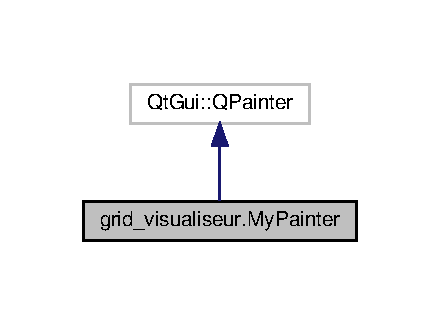
\includegraphics[width=211pt]{classgrid__visualiseur_1_1MyPainter__inherit__graph}
\end{center}
\end{figure}


Graphe de collaboration de grid\+\_\+visualiseur.\+My\+Painter\+:
\nopagebreak
\begin{figure}[H]
\begin{center}
\leavevmode
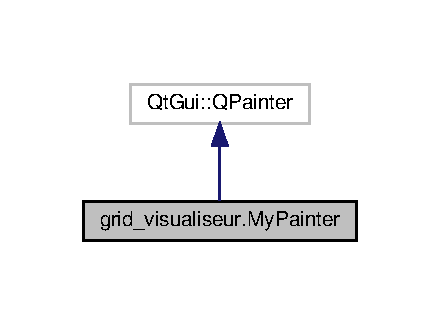
\includegraphics[width=211pt]{classgrid__visualiseur_1_1MyPainter__coll__graph}
\end{center}
\end{figure}
\subsection*{Fonctions membres publiques}
\begin{DoxyCompactItemize}
\item 
\mbox{\Hypertarget{classgrid__visualiseur_1_1MyPainter_ab6f7820d87cbc1b481f2055e44559cf1}\label{classgrid__visualiseur_1_1MyPainter_ab6f7820d87cbc1b481f2055e44559cf1}} 
def {\bfseries \+\_\+\+\_\+init\+\_\+\+\_\+} (self, scale, args, kwargs)
\item 
\mbox{\Hypertarget{classgrid__visualiseur_1_1MyPainter_a0a9785ebee0d148222e2895303b053b1}\label{classgrid__visualiseur_1_1MyPainter_a0a9785ebee0d148222e2895303b053b1}} 
def {\bfseries draw\+Pixmap} (self, x, y, image)
\end{DoxyCompactItemize}
\subsection*{Attributs publics}
\begin{DoxyCompactItemize}
\item 
\mbox{\Hypertarget{classgrid__visualiseur_1_1MyPainter_a8edb92d9f22e2fbdf9a12e70033f6e66}\label{classgrid__visualiseur_1_1MyPainter_a8edb92d9f22e2fbdf9a12e70033f6e66}} 
{\bfseries scale}
\end{DoxyCompactItemize}


La documentation de cette classe a été générée à partir du fichier suivant \+:\begin{DoxyCompactItemize}
\item 
grid\+\_\+visualiseur.\+py\end{DoxyCompactItemize}

\hypertarget{classqlearn_1_1Qlearner}{}\section{Référence de la classe qlearn.\+Qlearner}
\label{classqlearn_1_1Qlearner}\index{qlearn.\+Qlearner@{qlearn.\+Qlearner}}
\subsection*{Fonctions membres publiques}
\begin{DoxyCompactItemize}
\item 
def \hyperlink{classqlearn_1_1Qlearner_a2358d27a7a8833adaf69138ceda4d7aa}{\+\_\+\+\_\+init\+\_\+\+\_\+} (self, game)
\item 
def \hyperlink{classqlearn_1_1Qlearner_aa5d2c9fb82ed55754cab3f485551ba22}{reward} (self, state, action)
\item 
def \hyperlink{classqlearn_1_1Qlearner_a21001f2c11418262b3b0cfc58fb91f72}{learn} (self, nb\+\_\+iter, mu=0.\+9, c=1, explore=1)
\end{DoxyCompactItemize}
\subsection*{Attributs publics}
\begin{DoxyCompactItemize}
\item 
\mbox{\Hypertarget{classqlearn_1_1Qlearner_a69b12b006548c4ea15e63f5e22af8708}\label{classqlearn_1_1Qlearner_a69b12b006548c4ea15e63f5e22af8708}} 
{\bfseries game}
\item 
\mbox{\Hypertarget{classqlearn_1_1Qlearner_a27bf7d240f5a715866a7dc249dd0bacb}\label{classqlearn_1_1Qlearner_a27bf7d240f5a715866a7dc249dd0bacb}} 
{\bfseries actions}
\item 
\mbox{\Hypertarget{classqlearn_1_1Qlearner_a2eba21289650ffb2d6fd99ecfac97e63}\label{classqlearn_1_1Qlearner_a2eba21289650ffb2d6fd99ecfac97e63}} 
{\bfseries encoder}
\item 
\mbox{\Hypertarget{classqlearn_1_1Qlearner_a8bbd7e43cb52617447d6ddb6b67aed79}\label{classqlearn_1_1Qlearner_a8bbd7e43cb52617447d6ddb6b67aed79}} 
{\bfseries state\+\_\+number}
\item 
\mbox{\Hypertarget{classqlearn_1_1Qlearner_ad83c3b921b20c82bd5e6aa3ac550b4a5}\label{classqlearn_1_1Qlearner_ad83c3b921b20c82bd5e6aa3ac550b4a5}} 
{\bfseries int\+\_\+to\+\_\+state}
\item 
\mbox{\Hypertarget{classqlearn_1_1Qlearner_a590de5eb34ceb094ad2ce575064a46c1}\label{classqlearn_1_1Qlearner_a590de5eb34ceb094ad2ce575064a46c1}} 
{\bfseries action\+\_\+number}
\item 
\mbox{\Hypertarget{classqlearn_1_1Qlearner_a85cd72fc90598ce1036f3bfbf1e19cc8}\label{classqlearn_1_1Qlearner_a85cd72fc90598ce1036f3bfbf1e19cc8}} 
{\bfseries qtable}
\end{DoxyCompactItemize}


\subsection{Documentation des constructeurs et destructeur}
\mbox{\Hypertarget{classqlearn_1_1Qlearner_a2358d27a7a8833adaf69138ceda4d7aa}\label{classqlearn_1_1Qlearner_a2358d27a7a8833adaf69138ceda4d7aa}} 
\index{qlearn\+::\+Qlearner@{qlearn\+::\+Qlearner}!\+\_\+\+\_\+init\+\_\+\+\_\+@{\+\_\+\+\_\+init\+\_\+\+\_\+}}
\index{\+\_\+\+\_\+init\+\_\+\+\_\+@{\+\_\+\+\_\+init\+\_\+\+\_\+}!qlearn\+::\+Qlearner@{qlearn\+::\+Qlearner}}
\subsubsection{\texorpdfstring{\+\_\+\+\_\+init\+\_\+\+\_\+()}{\_\_init\_\_()}}
{\footnotesize\ttfamily def qlearn.\+Qlearner.\+\_\+\+\_\+init\+\_\+\+\_\+ (\begin{DoxyParamCaption}\item[{}]{self,  }\item[{}]{game }\end{DoxyParamCaption})}

\begin{DoxyVerb}construit un apprenant pour le jeu game 
\end{DoxyVerb}
 

\subsection{Documentation des fonctions membres}
\mbox{\Hypertarget{classqlearn_1_1Qlearner_a21001f2c11418262b3b0cfc58fb91f72}\label{classqlearn_1_1Qlearner_a21001f2c11418262b3b0cfc58fb91f72}} 
\index{qlearn\+::\+Qlearner@{qlearn\+::\+Qlearner}!learn@{learn}}
\index{learn@{learn}!qlearn\+::\+Qlearner@{qlearn\+::\+Qlearner}}
\subsubsection{\texorpdfstring{learn()}{learn()}}
{\footnotesize\ttfamily def qlearn.\+Qlearner.\+learn (\begin{DoxyParamCaption}\item[{}]{self,  }\item[{}]{nb\+\_\+iter,  }\item[{}]{mu = {\ttfamily 0.9},  }\item[{}]{c = {\ttfamily 1},  }\item[{}]{explore = {\ttfamily 1} }\end{DoxyParamCaption})}

\begin{DoxyVerb}apprend la Qtable en simulant nb_iter épisodes de jeu
mu est le facteur de récompense retardée
c le facteur d'apprentissage qui peut varier entre 0 et 1
c = 0 , l'agent n'apprend rien, 
c = 1 , l'agent met à jour complétement la valeur de Q (voir rapport)

explore est le facteur d'exploration qui peut varier entre 0 et 1 :
explore = 0  : l'agent choisit l'action à partir de la meilleure récompense dans la table
explore = 1 : l'agent explore en choisissant toutes ses actions au hasard
\end{DoxyVerb}
 \mbox{\Hypertarget{classqlearn_1_1Qlearner_aa5d2c9fb82ed55754cab3f485551ba22}\label{classqlearn_1_1Qlearner_aa5d2c9fb82ed55754cab3f485551ba22}} 
\index{qlearn\+::\+Qlearner@{qlearn\+::\+Qlearner}!reward@{reward}}
\index{reward@{reward}!qlearn\+::\+Qlearner@{qlearn\+::\+Qlearner}}
\subsubsection{\texorpdfstring{reward()}{reward()}}
{\footnotesize\ttfamily def qlearn.\+Qlearner.\+reward (\begin{DoxyParamCaption}\item[{}]{self,  }\item[{}]{state,  }\item[{}]{action }\end{DoxyParamCaption})}

\begin{DoxyVerb}    récompense liée à une action
    Si l'action ne fait pas changer d'état la récompense est -1
    Si l'action fait aboutir à un état final la récompense est 1
    Sinon la récompense est 0
    Après l'appel de cette fonction le jeu est dans le nouvel etat 
\end{DoxyVerb}
 

La documentation de cette classe a été générée à partir du fichier suivant \+:\begin{DoxyCompactItemize}
\item 
qlearn.\+py\end{DoxyCompactItemize}

\hypertarget{classrcolors_1_1RColors}{}\section{Référence de la classe rcolors.\+R\+Colors}
\label{classrcolors_1_1RColors}\index{rcolors.\+R\+Colors@{rcolors.\+R\+Colors}}


Graphe d\textquotesingle{}héritage de rcolors.\+R\+Colors\+:
\nopagebreak
\begin{figure}[H]
\begin{center}
\leavevmode
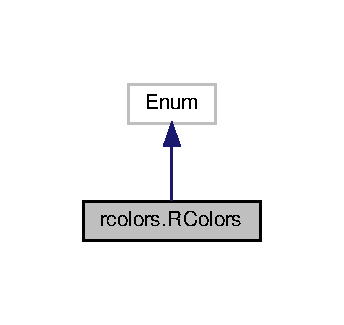
\includegraphics[width=165pt]{classrcolors_1_1RColors__inherit__graph}
\end{center}
\end{figure}


Graphe de collaboration de rcolors.\+R\+Colors\+:
\nopagebreak
\begin{figure}[H]
\begin{center}
\leavevmode
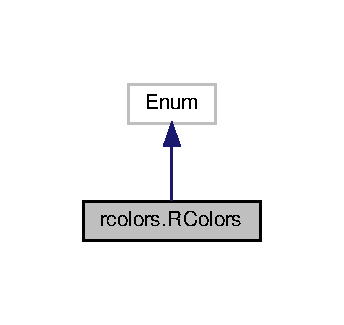
\includegraphics[width=165pt]{classrcolors_1_1RColors__coll__graph}
\end{center}
\end{figure}
\subsection*{Fonctions membres publiques}
\begin{DoxyCompactItemize}
\item 
\mbox{\Hypertarget{classrcolors_1_1RColors_ab8014c6c1a797ab32c7aa78633efb708}\label{classrcolors_1_1RColors_ab8014c6c1a797ab32c7aa78633efb708}} 
def {\bfseries \+\_\+\+\_\+str\+\_\+\+\_\+} (self)
\item 
\mbox{\Hypertarget{classrcolors_1_1RColors_a05522a9a34974e215921dc130cba1ded}\label{classrcolors_1_1RColors_a05522a9a34974e215921dc130cba1ded}} 
def {\bfseries from\+\_\+str} (cls, string)
\end{DoxyCompactItemize}
\subsection*{Attributs publics statiques}
\begin{DoxyCompactItemize}
\item 
\mbox{\Hypertarget{classrcolors_1_1RColors_a9ec86ff4d44cd118db70f93acf332939}\label{classrcolors_1_1RColors_a9ec86ff4d44cd118db70f93acf332939}} 
int {\bfseries R\+ED} = 1
\item 
\mbox{\Hypertarget{classrcolors_1_1RColors_a46f9f9493294a3e212d1b1d6a9381544}\label{classrcolors_1_1RColors_a46f9f9493294a3e212d1b1d6a9381544}} 
int {\bfseries G\+R\+E\+EN} = 2
\item 
\mbox{\Hypertarget{classrcolors_1_1RColors_af2153d6d9875761b8f0ee0726d514cfb}\label{classrcolors_1_1RColors_af2153d6d9875761b8f0ee0726d514cfb}} 
int {\bfseries B\+L\+UE} = 3
\item 
\mbox{\Hypertarget{classrcolors_1_1RColors_ae00773aea9e54ddca78695010ec40b67}\label{classrcolors_1_1RColors_ae00773aea9e54ddca78695010ec40b67}} 
int {\bfseries Y\+E\+L\+L\+OW} = 4
\end{DoxyCompactItemize}


La documentation de cette classe a été générée à partir du fichier suivant \+:\begin{DoxyCompactItemize}
\item 
rcolors.\+py\end{DoxyCompactItemize}

\hypertarget{classrobot_1_1Robot}{}\section{Référence de la classe robot.\+Robot}
\label{classrobot_1_1Robot}\index{robot.\+Robot@{robot.\+Robot}}
\subsection*{Fonctions membres publiques}
\begin{DoxyCompactItemize}
\item 
\mbox{\Hypertarget{classrobot_1_1Robot_a79a4241cf6242acb65cd51b1c67dd263}\label{classrobot_1_1Robot_a79a4241cf6242acb65cd51b1c67dd263}} 
def {\bfseries \+\_\+\+\_\+init\+\_\+\+\_\+} (self, group, color, position)
\item 
def \hyperlink{classrobot_1_1Robot_a10d00e1924a0fce095fe0bdf888f1415}{\+\_\+\+\_\+str\+\_\+\+\_\+} (self)
\item 
\mbox{\Hypertarget{classrobot_1_1Robot_a0227c4a66b9a23adb02a9ddf441be825}\label{classrobot_1_1Robot_a0227c4a66b9a23adb02a9ddf441be825}} 
def {\bfseries move} (self, dir, board)
\end{DoxyCompactItemize}
\subsection*{Attributs publics}
\begin{DoxyCompactItemize}
\item 
\mbox{\Hypertarget{classrobot_1_1Robot_a3ad797bc28203e41705888907ccf1958}\label{classrobot_1_1Robot_a3ad797bc28203e41705888907ccf1958}} 
{\bfseries group}
\item 
\mbox{\Hypertarget{classrobot_1_1Robot_ac6f9cffab22675391c0726d78efa6e70}\label{classrobot_1_1Robot_ac6f9cffab22675391c0726d78efa6e70}} 
{\bfseries color}
\item 
\mbox{\Hypertarget{classrobot_1_1Robot_ac276dce901ab21472c05818cf7b44383}\label{classrobot_1_1Robot_ac276dce901ab21472c05818cf7b44383}} 
{\bfseries position}
\end{DoxyCompactItemize}


\subsection{Documentation des fonctions membres}
\mbox{\Hypertarget{classrobot_1_1Robot_a10d00e1924a0fce095fe0bdf888f1415}\label{classrobot_1_1Robot_a10d00e1924a0fce095fe0bdf888f1415}} 
\index{robot\+::\+Robot@{robot\+::\+Robot}!\+\_\+\+\_\+str\+\_\+\+\_\+@{\+\_\+\+\_\+str\+\_\+\+\_\+}}
\index{\+\_\+\+\_\+str\+\_\+\+\_\+@{\+\_\+\+\_\+str\+\_\+\+\_\+}!robot\+::\+Robot@{robot\+::\+Robot}}
\subsubsection{\texorpdfstring{\+\_\+\+\_\+str\+\_\+\+\_\+()}{\_\_str\_\_()}}
{\footnotesize\ttfamily def robot.\+Robot.\+\_\+\+\_\+str\+\_\+\+\_\+ (\begin{DoxyParamCaption}\item[{}]{self }\end{DoxyParamCaption})}

\begin{DoxyVerb}renvoie une représentation du robot sous forme de chaîne de caractères
    "R" : [x,y]
\end{DoxyVerb}
 

La documentation de cette classe a été générée à partir du fichier suivant \+:\begin{DoxyCompactItemize}
\item 
robot.\+py\end{DoxyCompactItemize}

\hypertarget{classrobot_1_1Robot__group}{}\section{Référence de la classe robot.\+Robot\+\_\+group}
\label{classrobot_1_1Robot__group}\index{robot.\+Robot\+\_\+group@{robot.\+Robot\+\_\+group}}


Graphe d\textquotesingle{}héritage de robot.\+Robot\+\_\+group\+:
\nopagebreak
\begin{figure}[H]
\begin{center}
\leavevmode
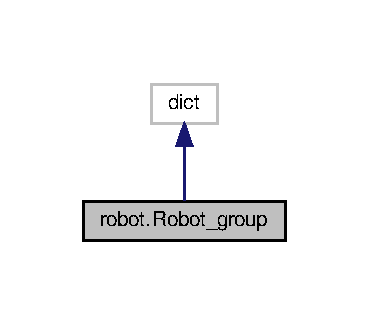
\includegraphics[width=177pt]{classrobot_1_1Robot__group__inherit__graph}
\end{center}
\end{figure}


Graphe de collaboration de robot.\+Robot\+\_\+group\+:
\nopagebreak
\begin{figure}[H]
\begin{center}
\leavevmode
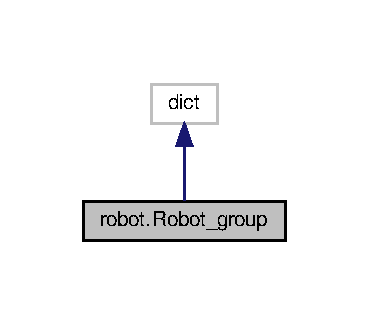
\includegraphics[width=177pt]{classrobot_1_1Robot__group__coll__graph}
\end{center}
\end{figure}
\subsection*{Fonctions membres publiques}
\begin{DoxyCompactItemize}
\item 
\mbox{\Hypertarget{classrobot_1_1Robot__group_aed143932a9520e3c8255b76933d7eb41}\label{classrobot_1_1Robot__group_aed143932a9520e3c8255b76933d7eb41}} 
def {\bfseries add\+\_\+robot} (self, robot)
\item 
\mbox{\Hypertarget{classrobot_1_1Robot__group_adbbbe6a28fbf51a4bfbb75ad83a85d33}\label{classrobot_1_1Robot__group_adbbbe6a28fbf51a4bfbb75ad83a85d33}} 
def {\bfseries cell\+\_\+occupied} (self, pos)
\item 
\mbox{\Hypertarget{classrobot_1_1Robot__group_abd35bb6cd4e236c25155231b8a56953a}\label{classrobot_1_1Robot__group_abd35bb6cd4e236c25155231b8a56953a}} 
def {\bfseries \+\_\+\+\_\+str\+\_\+\+\_\+} (self)
\end{DoxyCompactItemize}


La documentation de cette classe a été générée à partir du fichier suivant \+:\begin{DoxyCompactItemize}
\item 
robot.\+py\end{DoxyCompactItemize}

\hypertarget{classsolveur_1_1solveur}{}\section{Référence de la classe solveur.\+solveur}
\label{classsolveur_1_1solveur}\index{solveur.\+solveur@{solveur.\+solveur}}
\subsection*{Fonctions membres publiques}
\begin{DoxyCompactItemize}
\item 
def \hyperlink{classsolveur_1_1solveur_aaac83179919b07e763025ea73d4ccce3}{\+\_\+\+\_\+init\+\_\+\+\_\+} (self, game)
\item 
def \hyperlink{classsolveur_1_1solveur_aae96bc7e6e7b11a51d4a55564414ba92}{find\+\_\+solution} (self)
\end{DoxyCompactItemize}
\subsection*{Fonctions membres publiques statiques}
\begin{DoxyCompactItemize}
\item 
def \hyperlink{classsolveur_1_1solveur_af3ccbdb13bf858ee950da16f2d736d52}{action\+\_\+sequence\+\_\+from\+\_\+pred} (pred, final\+\_\+state, initial\+\_\+state)
\end{DoxyCompactItemize}
\subsection*{Attributs publics}
\begin{DoxyCompactItemize}
\item 
\mbox{\Hypertarget{classsolveur_1_1solveur_ad73a71390ca87152dc67d4f0855675ee}\label{classsolveur_1_1solveur_ad73a71390ca87152dc67d4f0855675ee}} 
{\bfseries game}
\end{DoxyCompactItemize}


\subsection{Documentation des constructeurs et destructeur}
\mbox{\Hypertarget{classsolveur_1_1solveur_aaac83179919b07e763025ea73d4ccce3}\label{classsolveur_1_1solveur_aaac83179919b07e763025ea73d4ccce3}} 
\index{solveur\+::solveur@{solveur\+::solveur}!\+\_\+\+\_\+init\+\_\+\+\_\+@{\+\_\+\+\_\+init\+\_\+\+\_\+}}
\index{\+\_\+\+\_\+init\+\_\+\+\_\+@{\+\_\+\+\_\+init\+\_\+\+\_\+}!solveur\+::solveur@{solveur\+::solveur}}
\subsubsection{\texorpdfstring{\+\_\+\+\_\+init\+\_\+\+\_\+()}{\_\_init\_\_()}}
{\footnotesize\ttfamily def solveur.\+solveur.\+\_\+\+\_\+init\+\_\+\+\_\+ (\begin{DoxyParamCaption}\item[{}]{self,  }\item[{}]{game }\end{DoxyParamCaption})}

\begin{DoxyVerb}crée un solveur pour game \end{DoxyVerb}
 

\subsection{Documentation des fonctions membres}
\mbox{\Hypertarget{classsolveur_1_1solveur_af3ccbdb13bf858ee950da16f2d736d52}\label{classsolveur_1_1solveur_af3ccbdb13bf858ee950da16f2d736d52}} 
\index{solveur\+::solveur@{solveur\+::solveur}!action\+\_\+sequence\+\_\+from\+\_\+pred@{action\+\_\+sequence\+\_\+from\+\_\+pred}}
\index{action\+\_\+sequence\+\_\+from\+\_\+pred@{action\+\_\+sequence\+\_\+from\+\_\+pred}!solveur\+::solveur@{solveur\+::solveur}}
\subsubsection{\texorpdfstring{action\+\_\+sequence\+\_\+from\+\_\+pred()}{action\_sequence\_from\_pred()}}
{\footnotesize\ttfamily def solveur.\+solveur.\+action\+\_\+sequence\+\_\+from\+\_\+pred (\begin{DoxyParamCaption}\item[{}]{pred,  }\item[{}]{final\+\_\+state,  }\item[{}]{initial\+\_\+state }\end{DoxyParamCaption})\hspace{0.3cm}{\ttfamily [static]}}

\begin{DoxyVerb}cette fonction reconstruit la sequence d'action menant de l'etat initial à l'etat final
en utilisant le tableau des predecesseurs
\end{DoxyVerb}
 \mbox{\Hypertarget{classsolveur_1_1solveur_aae96bc7e6e7b11a51d4a55564414ba92}\label{classsolveur_1_1solveur_aae96bc7e6e7b11a51d4a55564414ba92}} 
\index{solveur\+::solveur@{solveur\+::solveur}!find\+\_\+solution@{find\+\_\+solution}}
\index{find\+\_\+solution@{find\+\_\+solution}!solveur\+::solveur@{solveur\+::solveur}}
\subsubsection{\texorpdfstring{find\+\_\+solution()}{find\_solution()}}
{\footnotesize\ttfamily def solveur.\+solveur.\+find\+\_\+solution (\begin{DoxyParamCaption}\item[{}]{self }\end{DoxyParamCaption})}

\begin{DoxyVerb}cette méthode détermine une solution utilisant un minimum d'actions
\end{DoxyVerb}
 

La documentation de cette classe a été générée à partir du fichier suivant \+:\begin{DoxyCompactItemize}
\item 
solveur.\+py\end{DoxyCompactItemize}

\hypertarget{classstateencoder_1_1StateEncoder}{}\section{Référence de la classe stateencoder.\+State\+Encoder}
\label{classstateencoder_1_1StateEncoder}\index{stateencoder.\+State\+Encoder@{stateencoder.\+State\+Encoder}}
\subsection*{Fonctions membres publiques}
\begin{DoxyCompactItemize}
\item 
\mbox{\Hypertarget{classstateencoder_1_1StateEncoder_a503f0aa0c6cfae6f022fd79fd2bfa152}\label{classstateencoder_1_1StateEncoder_a503f0aa0c6cfae6f022fd79fd2bfa152}} 
def {\bfseries \+\_\+\+\_\+init\+\_\+\+\_\+} (self, game)
\item 
\mbox{\Hypertarget{classstateencoder_1_1StateEncoder_aff259f1e3d3e79919557b75aac758054}\label{classstateencoder_1_1StateEncoder_aff259f1e3d3e79919557b75aac758054}} 
def {\bfseries position\+\_\+encoder\+\_\+functions} (self)
\item 
\mbox{\Hypertarget{classstateencoder_1_1StateEncoder_a1ccde118fbd3eccb9dde2610533c9dae}\label{classstateencoder_1_1StateEncoder_a1ccde118fbd3eccb9dde2610533c9dae}} 
def {\bfseries state\+\_\+index\+\_\+function} (self)
\end{DoxyCompactItemize}
\subsection*{Attributs publics}
\begin{DoxyCompactItemize}
\item 
\mbox{\Hypertarget{classstateencoder_1_1StateEncoder_af55cb60af3c00cb2ff576163046fb672}\label{classstateencoder_1_1StateEncoder_af55cb60af3c00cb2ff576163046fb672}} 
{\bfseries game}
\item 
\mbox{\Hypertarget{classstateencoder_1_1StateEncoder_a0db3da25383e1889ac047aedad6aee8f}\label{classstateencoder_1_1StateEncoder_a0db3da25383e1889ac047aedad6aee8f}} 
{\bfseries state\+\_\+number}
\end{DoxyCompactItemize}


La documentation de cette classe a été générée à partir du fichier suivant \+:\begin{DoxyCompactItemize}
\item 
stateencoder.\+py\end{DoxyCompactItemize}

%--- End generated contents ---

% Index
\backmatter
\newpage
\phantomsection
\clearemptydoublepage
\addcontentsline{toc}{chapter}{Index}
\printindex

\end{document}
